% **************************************************************************** %
\chapter{\"Uberblick}
\label{chap:uberblick}
% **************************************************************************** %

In   diesem  Kapitel   wird  zuerst   kurz  der   grundlegende  Aufbau   einer
PV-Anlage  erkl\"art,  um   sicherzustellen,  dass  keine  Missverst\"andnisse
beim   Interpretieren    der   nachfolgenden   Informationen   und    in   der
verwendeten Terminologie entstehen. Anschliessend werden Simulationsergebnisse
pr\"asentiert,   welche  verdeutlichen,   dass  die   Leistungsverluste  durch
einzelne,  nicht  optimal  funktionierende  Zellen  in  einer  grossen  Anlage
im  Bereich   von  mehreren  Kilowatt  liegen   k\"onnen. Daraus  leitet  sich
schlussendlich  die  Notwendigkeit   eines  \"Uberwachungssystems  ab. Zuletzt
werden verschiedene  Varianten vorgestellt,  wie ein  Signal auf  den DC-Strom
in   der  Leitung   zwischen   PV-Modul  und   Zentrale  aufmoduliert   werden
kann: Frequenzumtastung, Amplitudenumtastung  und \emph{On-off Keying}.


% ---------------------------------------------------------------------------- %
\section{Aufbau einer Photovoltaikanlage}
\label{sec:solaranlage:aufbau}
% ---------------------------------------------------------------------------- %

\enlargethispage{1em}
\begin{wrapfigure}{r}{0.35\textwidth}
    \centering
    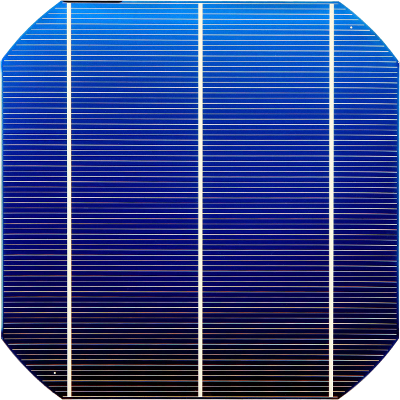
\includegraphics[width=0.30\textwidth]{images/solar-facility/cell--400px.png}
    \caption[Bild einer PV-Zelle]
    {Solarzelle, Frontalansicht \cite{ref:pvcell:wikipedia}}
    \label{fig:pvcell:front}
    \vspace*{-1em}
\end{wrapfigure}

Die   Grundbausteine    einer   Photovoltaikanlage   legen    die   PV-Zellen,
welche   aus   verschiedenen   Halbleitermaterialien   bestehen. Die   meisten
heutzutage  verwendeten  Zellen  werden aus  dem  Halbleitermaterial  Silizium
hergestellt. Siliziumzellen  sind in  verschiedenen Formfaktoren  verf\"ugbar;
g\"angige   Gr\"ossen    haben   ca.   zwischen    \SI{10}{\centi\meter}   und
\SI{15}{\centi\meter}  Kantenl\"ange.   Zum  mechanischen  Schutz  der  Zellen
sind  diese mit  einer durchsichtigen  Antireflexschicht \"uberzogen.   Die an
der  PV-Zelle  abgreifbare  Spannung betr\"agt  zwischen  \SI{0.5}{\volt}  und
\SI{0.8}{\volt} DC,  wobei die  Klemmenspannung einer  voll funktionsf\"ahigen
Zelle nur schwach von  der Lichteinstrahlung abh\"angig ist. Die Stromst\"arke
hingegen   ist  sehr   stark  von   der  Beleuchtungsst\"arke   abh\"angig. Je
nach    Sonneneinstrahlung   erreicht    eine   \SI{100}{\centi\meter\squared}
grosse   Siliziumzelle  eine   Stromst\"arke   von   bis  zu   \SI{2}{\ampere}
\cite{ref:pv:gesellschaftFuerSonnenenergie}. \fref{fig:pvcell:front} zeigt die
Frontansicht einer PV-Zelle.

\clearpage
\begin{wrapfigure}{l}{0.45\textwidth}
    \centering
    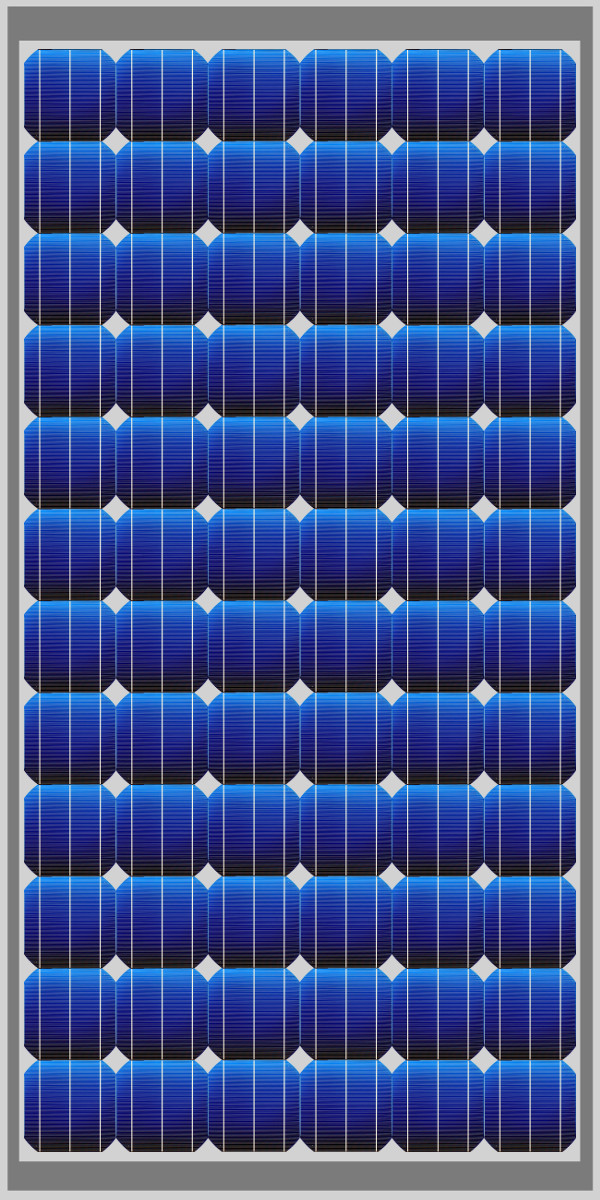
\includegraphics[width=0.4\textwidth]{images/solar-facility/pvmodule.jpeg}
    \caption[Bild eines PV-Moduls]
    {%
        Solarmodul,  zusammengesetzt  aus  72 Solarzellen  gem\"ass  Abbildung
        \ref{fig:pvcell:front}%
    }
    \label{fig:pvmodule}
    \vspace*{-1em}
\end{wrapfigure}


Die  in der  Praxis  \"ubliche  Baugruppe ist  nicht  die Solarzelle,  sondern
das   Photovoltaikmodul.\hfill   Um   \hfill   die   \hfill   Ausgangsspannung
\\und/oder  den  Ausgangsstrom  zu  erh\"ohen  und  um  diese  in  der  Praxis
besser  einsetzen   zu  k\"onnen,  werden  mehrere   Zellen  in  verschiedenen
Konfigurationen  miteinander zu  einem PV-Modul  verschaltet. Das Konzept  ist
schematisch dargestellt in Abbildung  \ref{fig:pvmodule}, die Eckdaten einiger
PV-Module sind als Beispiele  in Anhang \ref{app:commercial:modules} auf Seite
\pageref{app:commercial:modules} aufgef\"uhrt.

Zur  Erh\"ohung  des Ausgangsstroms  werden  Zellen  parallel geschaltet,  zur
Erh\"ohung  der  Ausgangsspannung werden  sie  in  Serie verbunden.   Je  nach
gew\"unschten Spezifikationen eines Moduls werden diese Ans\"atze einzeln oder
kombiniert angewandt.  In der Praxis \"ublich  sind Module mit 36, 72 oder 144
Zellen und  einer Ausgangsspannung  von \SI{12}{\volt}  bis \SI{60}{\volt}. In
Photovoltaikanlagen werden nur solche  ganzen Module eingesetzt; die einzelnen
Zellen  sind  f\"ur  Reparaturen  nicht  mehr  zug\"anglich. Die  elektrischen
Anschl\"usse befinden sich in kleinen  Kunststoffdosen auf der R\"uckseite der
Module (Beispiel in Abbildung \ref{fig:pvJunctionBox}) \cite{ref:pv:baunetz}.


Mehrere  identische  Module  werden  \"ublicherweise  mittels  Reihenschaltung
zu  einem  Modulstrang  verschaltet   (vereinfacht  dargestellt  in  Abbildung
\ref{fig:pvarray:gak:inverter}).  Dadurch wird  eine h\"ohere Ausgangsspannung
erzeugt, was die Umwandlung des Gleichstroms in

\begin{wrapfigure}{r}{0.35\textwidth}
    \centering
    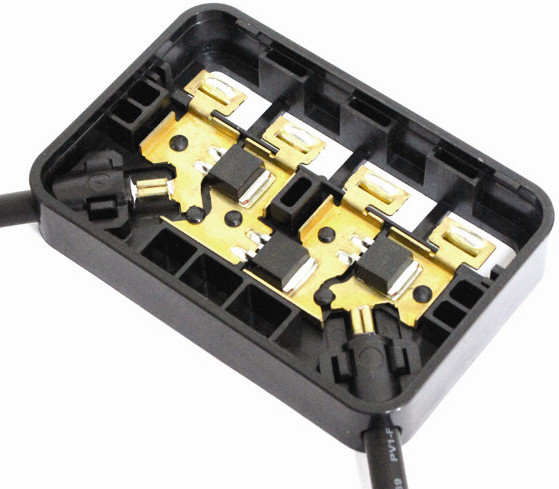
\includegraphics[width=0.3\textwidth]{images/solar-facility/pvJunctionBox.jpeg}
    \caption[Anschlussbox PV-Modul]{
        Anschlussbox   f\"ur   PV-Modul,   Montage   normalerweise   auf   der
        R\"uckseite  des  Moduls  \cite{ref:junctionBox}. Es  sind  auch  drei
        Freilaufdioden  erkennbar  (Abschnitt \ref{sec:shadedCells}  ab  Seite
        \pageref{sec:shadedCells})%
    }
    \label{fig:pvJunctionBox}
\end{wrapfigure}

\noindent   Wechselstrom   und   dessen   Einspeisung   ins   Wechselstromnetz
erleichtert. Die Ausgangsspannung eines  Modulstrangs darf gem\"ass Vorschrift
\SI{1000}{\volt} DC nicht \"uberschreiten, was  die Anzahl der in einem Strang
in Serie  geschalteten Module beschr\"ankt.  Module,  die an unterschiedlichen
Dachneigungen  montiert sind  oder die  unterschiedliche Ausrichtungen  haben,
sollten nie zu  einem Modulstrang zusammengeschaltet werden, da  sie nicht den
gleichen  Strom  produzieren  werden,  was die  Effizienz  des  Strangs  stark
reduziert. Ein einzelnes beschattetes  oder nicht einwandfrei funktionierendes
Modul beeintr\"achtigt die vom  gesamten Modulstrang abgegebene Leistung stark
(siehe n\"achster Abschnitt).

\clearpage
\enlargethispage{2em}
\begin{figure}[h!t]
    \centering
    \begin{tikzpicture}
        \begin{scope}[x={(0mm,\textwidth)},y={(0mm,-70mm)}]
            \node[inner sep=0pt,anchor=north west] at (0mm,0mm) {%
                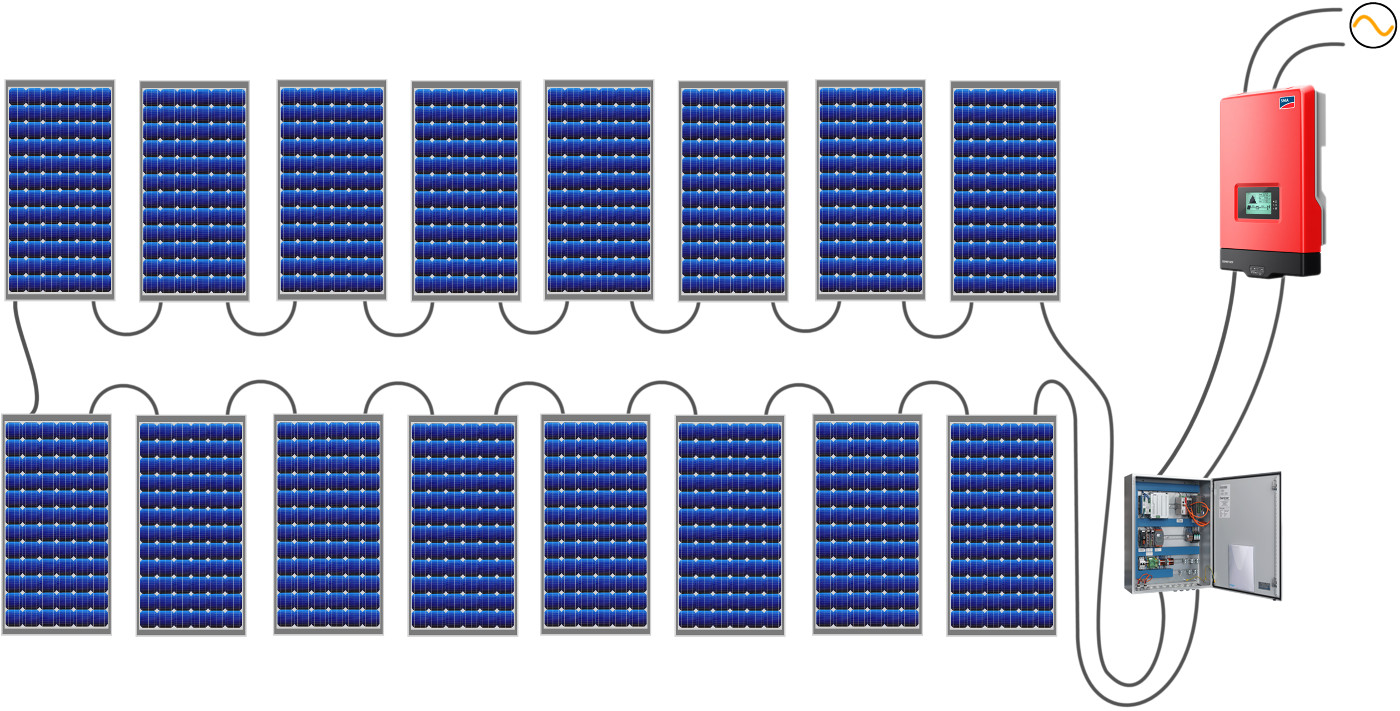
\includegraphics[width=\textwidth]{images/solar-facility/pvarray.jpeg}%
            };
            \node at (132mm,-55mm) {\small{GAK}};
            \node at (120mm,0mm) {\small{Wechselrichter}};
            \node at (55mm,-5mm) {\small{Modulstrang}};
        \end{scope}
    \end{tikzpicture}
    \caption[Modulstrang, \"Ubersichtsbild]{%
        Modulstrang aus 16 Modulen  gem\"ass Abbildung \ref{fig:pvmodule}, GAK
        und Wechselrichter. Bild des GAK  von \cite{ref:gak:gantner}, Bild des
        Wechselrichters von \cite{ref:inverter:sunnyboy}.%
    }
    \label{fig:pvarray:gak:inverter}
\end{figure}

Die    Umwandlung    der    Gleichspannung    in    Wechselspannung    erfolgt
mittels    Wechselrichter   (dargestellt    auf   der    rechten   Seite    in
Abbildung  \ref{fig:pvarray:gak:inverter}). Je  nach Anwendungsbereich  werden
unterschiedliche   Wechselrichter    eingesetzt,   aufgelistet    in   Tabelle
\ref{tab:inverters}.

\begin{table}[h!tb]
    \centering
    \caption{Arten von Wechselrichtern}
    \label{tab:inverters}
    \begin{tabular}{p{50mm}p{70mm}}
        \toprule
        \textbf{Modulwechselrichter}: &
        Ein  Wechselrichter,  welcher  den  Strom eines  einzelnen  Moduls  in
        Wechselstrom konvertiert. \\

        \textbf{Strangwechselrichter}: &
        Konvertiert den Strom eines Modulstrangs zu Wechselstrom. \\

        \textbf{Multistrangwechselrichter}: &
        Fasst   die   Gleichstr\"ome   mehrer  Modulstr\"ange   zusammen   und
        konvertiert diese zu Wechselstrom. \\

        \textbf{Zentralwechselrichter}: &
        Ein  einzelner Wechselrichter,  welcher den  Gleichstrom einer  ganzen
        Photovoltaikanlage in Wechselstrom umwandelt. Kommt haupts\"achlich in
        Grossanlagen zum Einsatz, bei denen alle Str\"ange die gleiche Neigung
        aufweisen und gleich ausgerichtet sind \cite{ref:pv:ratgeber}.\\
        \bottomrule
    \end{tabular}
\end{table}

Als Leitungsschutz gegen \"Uberstrom und Kurzschluss befindet sich unmittelbar
vor  dem   Wechselrichter  im  Gleichstromnetz   ein  Generatoranschlusskasten
(GAK). Dieser   dient   auch   zur    Trennung   der   gesamten   Anlage   vom
Netz. \"Ublicherweise  werden  GAK  und   Wechselrichter  am  selben  Standort
platziert.


% ---------------------------------------------------------------------------- %
\clearpage
\section{Leistungseinbr\"uche}
\label{sec:shadedCells}
% ---------------------------------------------------------------------------- %

In  diesem Abschnitt  werden einige  Simulationsergebnisse pr\"asentiert,  die
exemplarisch zeigen,  wie drastisch  die Leistungsf\"ahigkeit  einer PV-Anlage
aufgrund von kleinen Ursachen abnehmen kann.

Bei  der  Serieschaltung   von  Zellen  zu  einem  Modul   kann  bereits  eine
einzelne   nicht   voll   funktionsf\"ahige   Zelle   zu   starken   Einbussen
bei   der   Leistungsf\"ahigkeit  des   Moduls   f\"uhren\footnotemark. Dieser
Effekt  ist  in   den  Abbildungen  \ref{fig:simu:iv-curves:module:generic:3d}
und    \ref{fig:simu:iv-curves:module:generic}     gezeigt. Die    Abbildungen
basieren   auf    der   Simulation    eines   PV-Moduls,   welches    aus   72
in   Serie   geschalteten   Zellen   besteht   (die   zugeh\"orige   Schaltung
ist    in    Abbildung     \ref{fig:ltspice:iv:generic:module}    auf    Seite
\pageref{fig:ltspice:iv:generic:module}  dargestellt). Gibt   schon  nur  eine
von  72 Zellen  weniger  Strom  ab als  die  restlichen,  verringert sich  die
Leistungsf\"ahigkeit des Moduls betr\"achtlich. Der dabei von einem Modul noch
abgegebene Strom h\"angt wesentlich vom  Shunt-Widerstand des Modells bzw. vom
parallelen Innenwiderstand  der Zelle  ab (mehr zum  Modell einer  PV-Zelle in
Abschnitt \ref{sec:simu:model:cell} ab Seite \pageref{sec:simu:model:cell}).

\footnotetext{%
    Es   sei   an   dieser   Stelle  noch   erw\"ahnt,   dass   aufgrund   von
    Fertigungstoleranzen bei  realen Modulen  nat\"urlich niemals  alle Zellen
    den genau gleichen Arbeitspunkt  haben. Diese Effekte zu ber\"ucksichtigen
    w\"urde jedoch  die im  Rahmen dieses  Projekts zur  Verf\"ugung stehenden
    Ressourcen \"ubersteigen. Daher werden sie  f\"ur den Rest dieses Berichts
    nicht ber\"ucksichtigt.%
}

\begin{figure}[h!tb]
    \centering
    \begin{tikzpicture}
   \begin{scope}[x={(0mm,120mm)},y={(0mm,100mm)}]
        \begin{axis}[
            %colormap/hot2,
            colormap/cool,
            %colormap/viridis,
            %colormap/temp,
            height=80mm,
            width=120mm,
            grid=both,
            zmin=0,
            thick,
            xlabel=Spannung,
            ylabel=Strom,
            zlabel=Leistung,
            legend style={at={(0,-0.15)},anchor=north west},
            legend cell align=left,
        ]
            % 10A
            \addplot3[
                %draw=blue,
                draw=blue,
                scatter src = \thisrow{I(R3)},
            ] table[y expr=9] {data/iv-curves/generic-module/iv-generic--9a.dat};
            \addplot3[
                %draw=blue,
                draw=blue,
                scatter src = \thisrow{power},
            ] table[x expr=47] {data/iv-curves/generic-module/iv-generic--9a.dat};
            \addplot3[
                %draw=blue,
                draw=blue,
                scatter src = \thisrow{power},
            ] table[x expr=0] {data/iv-curves/generic-module/iv-generic--9a.dat};
            \addplot3[
                %draw=blue,
                draw=blue,
                scatter src = \thisrow{I(R3)},
            ] table[z expr=0] {data/iv-curves/generic-module/iv-generic--9a.dat};
            \addplot3[
                surf,
                shader=interp,
            ] table {data/iv-curves/generic-module/iv-generic--full-dataset.dat};
            \addplot3[
                draw=blue,
                very thick,
            ] table {data/iv-curves/generic-module/iv-generic--full-dataset.dat};
        \end{axis}
    \end{scope}
\end{tikzpicture}

    \caption
    [3d-Darstellung von Leistung, Spannung und Strom eines PV-Moduls]
    {%
        3D-Darstellung  von  Leistung,  Spannung und  Strom  eines  PV-Moduls.
        Abbildung    \ref{fig:simu:iv-curves:module:generic}    zeigt    diese
        Kurven  zweidimensional.    Die  zuge\"orige  \code{LTspice}-Schaltung
        ist   in  Abbildung   \ref{fig:ltspice:iv:generic:module}  auf   Seite
        \pageref{fig:ltspice:iv:generic:module} abgebildet.%
    }
    \label{fig:simu:iv-curves:module:generic:3d}
\end{figure}

\begin{figure}[h!tb]
    \centering
    \begin{tikzpicture}
   \begin{scope}[x={(0mm,0mm)},y={(90mm,0.9\textwidth)}]
       \begin{axis}[%
               height=50mm,
               width=\textwidth,
               at={(0,50mm)},
               grid=both,
               xlabel=Spannung (\si{\volt}),
               ylabel=Strom (\si{\ampere}),
               colormap/hot2,
               %axis y line*=left,
               %x unit=u,
               %change x base=true,
               %line width = 1pt,
               %thick,
               %x SI prefix=micro,
           ]
           \addplot[-,purple]  table[x=V(out), y=I(R3)] {data/iv-curves/generic-module/iv-generic--1a.dat};
           \addplot[-,teal]    table[x=V(out), y=I(R3)] {data/iv-curves/generic-module/iv-generic--4a.dat};
           \addplot[-,magenta] table[x=V(out), y=I(R3)] {data/iv-curves/generic-module/iv-generic--7a.dat};
           \addplot[-,blue]    table[x=V(out), y=I(R3)] {data/iv-curves/generic-module/iv-generic--9a.dat};
            %\addplot[-,color=blue] table {data/iv-curves/module-72cells-series--reference--all-ok.dat};
            %\addplot[-,color=teal] table {data/iv-curves/module-72cells-series--reference--ifail-5A.dat};
            %\addplot[-,color=magenta] table {data/iv-curves/module-72cells-series--reference--ifail-1A.dat};
        \end{axis}
        \begin{axis}[%
               height=50mm,
               width=\textwidth,
               at={(0,0)},
               grid=both,
               xlabel=Spannung (\si{\volt}),
               ylabel=Leistung (\si{\watt}),
               %axis y line*=left,
               %x unit=u,
               %change x base=true,
               %line width = 1pt,
               %thick,
               %x SI prefix=micro,
           ]
           \addplot[-,purple]  table[x=V(out), y=power] {data/iv-curves/generic-module/iv-generic--1a.dat};
           \addplot[-,teal]    table[x=V(out), y=power] {data/iv-curves/generic-module/iv-generic--4a.dat};
           \addplot[-,magenta] table[x=V(out), y=power] {data/iv-curves/generic-module/iv-generic--7a.dat};
           \addplot[-,blue]    table[x=V(out), y=power] {data/iv-curves/generic-module/iv-generic--9a.dat};
        \end{axis}
    \end{scope}
\end{tikzpicture}

    \caption[IV- und PV-Kurven eines PV-Moduls bei Leistungseinbruch]{%
        Verhalten   eines    Moduls   bei    Reduktion   des    Stroms   einer
        einzelnen   Zelle.
        Die   zuge\"orige  \code{LTspice}-Schaltung   ist
        in    Abbildung    \ref{fig:ltspice:iv:generic:module}    auf    Seite
        \pageref{fig:ltspice:iv:generic:module}    zu    finden.     Abbildung
        \ref{fig:simu:iv-curves:module:generic:3d}  zeigt  die  entsprechenden
        Zusammenh\"ange dreidimensional.%
    }
    \label{fig:simu:iv-curves:module:generic}
\end{figure}

Bei Serieschaltung von  mehreren PV-Modulen in einem Strang  kann bereits eine
einzige nicht  voll funktionsf\"ahige  Zelle in einem  Modul die  Leistung des
gesamten Strangs  stark beeintr\"achtigen.   Der gesamte  von einem  Modul und
somit auch von einem Strang (wegen Serieschaltung der Module) abgegebene Strom
h\"angt also stark von der schw\"achsten Zelle in der Schaltung ab.

Um  diesen  Effekt  zu  reduzieren,  werden  in  der  Praxis  in  jedem  Modul
jeweils  \"uber mehreren  Zellen  Freilaufdioden  (Engl. \emph{Bypass  Diode})
geschaltet. In  der  Anschlussbox  aus Abbildung  \ref{fig:pvJunctionBox}  von
Seite \pageref{fig:pvJunctionBox} sind drei Freilaufdioden sichtbar, womit zum
Beispiel drei  mal 24  Zellen mit je  einer Freilaufdiode  parallel geschaltet
werden k\"onnten. Aus Kostengr\"unden wird  nicht eine Freilaufdiode pro Zelle
verbaut, obwohl dies aus elektrotechnischer Sicht optimal w\"are.

\clearpage
Wird   ein   Strom   durch   eine   PV-Zelle   geleitet,   ohne   dass   diese
gen\"ugend   belichtet   ist,   findet    \"uber   der   Zelle   statt   eines
Spannungsanstiegs   wie    im   regul\"aren   Betrieb    ein   Spannungsabfall
statt,  was   bedeutet,  dass   der  durch   die  PV-Zelle   fliessende  Strom
in   der   Zelle   thermische   Verluste  produziert. Dies   ist   nicht   nur
ineffizient   und  un\"okonomisch,   sondern   kann   auch  eine   Brandgefahr
darstellen. Abbildung    \ref{fig:simu:iv-curves:array:generic}   zeigt    die
Simulation eines  Modulstrangs, in  dem keines  der Module  mit Freilaufdioden
versehen  ist. Wie  leicht  zu  erkennen  ist,  f\"allt  die  vom  Modulstrang
abgegebene Leistung bereits bei einer einzigen defekten Zelle (von 1440 Zellen
im gesamten Modulstrang!)  bedeutend ab. Gibt eine Zelle  lediglich noch einen
F\"unftel  des Stromes  der restlichen  Zellen  ab, f\"allt  die vom  gesamten
Strang  abgegebene Leistung  um etwa  einen Viertel. Da  die Sonneneintrahlung
verglichen mit  einer voll  funktionsf\"ahigen Anlage aber  unver\"andert ist,
produziert die Anlage eigentlich immer noch beinahge gleich viel Leistung. Die
nicht  mehr  zur  Verf\"ugung  stehende  Leistung  wird  aber  gr\"osstenteils
thermisch statt elektrisch abgegeben (daher auch Brandgefahr).


\begin{figure}[h!tb]
    \centering
    \begin{tikzpicture}
   \begin{scope}[x={(0mm,0mm)},y={(90mm,0.9\textwidth)}]
       \begin{axis}[%
               height=50mm,
               width=\textwidth,
               at={(0,50mm)},
               grid=both,
               xlabel=Spannung (\si{\volt}),
               ylabel=Strom (\si{\ampere}),
               colormap/hot2,
               %axis y line*=left,
               %x unit=u,
               %change x base=true,
               %line width = 1pt,
               %thick,
               %x SI prefix=micro,
           ]
           \addplot[-,purple]  table[x=V(out), y=I(R3)] {data/iv-curves/generic-array/iv-generic--1a.dat};
           \addplot[-,teal]    table[x=V(out), y=I(R3)] {data/iv-curves/generic-array/iv-generic--4a.dat};
           \addplot[-,magenta] table[x=V(out), y=I(R3)] {data/iv-curves/generic-array/iv-generic--7a.dat};
           \addplot[-,blue]    table[x=V(out), y=I(R3)] {data/iv-curves/generic-array/iv-generic--9a.dat};
            %\addplot[-,color=blue] table {data/iv-curves/module-72cells-series--reference--all-ok.dat};
            %\addplot[-,color=teal] table {data/iv-curves/module-72cells-series--reference--ifail-5A.dat};
            %\addplot[-,color=magenta] table {data/iv-curves/module-72cells-series--reference--ifail-1A.dat};
        \end{axis}
        \begin{axis}[%
               height=50mm,
               width=\textwidth,
               at={(0,0)},
               grid=both,
               xlabel=Spannung (\si{\volt}),
               ylabel=Leistung (\si{\watt}),
               %axis y line*=left,
               %x unit=u,
               %change x base=true,
               %line width = 1pt,
               %thick,
               %x SI prefix=micro,
           ]
           \addplot[-,purple]  table[x=V(out), y=power] {data/iv-curves/generic-array/iv-generic--1a.dat};
           \addplot[-,teal]    table[x=V(out), y=power] {data/iv-curves/generic-array/iv-generic--4a.dat};
           \addplot[-,magenta] table[x=V(out), y=power] {data/iv-curves/generic-array/iv-generic--7a.dat};
           \addplot[-,blue]    table[x=V(out), y=power] {data/iv-curves/generic-array/iv-generic--9a.dat};
        \end{axis}
    \end{scope}
\end{tikzpicture}

    \caption[%
        IV- und PV-Kurven eines Modulsstrangs bei Leistungseinbruch,
        keine Freilaufdioden%
    ]
    {%
        Verhalten       eines      Modulstrangs       ohne      Freilaufdioden
        bei     Reduktion     des     Stroms    einer     einzelnen     Zelle.
        Die      zugeh\"origen     \code{LTspice}-Schaltungen      sind     im
        Anhang       in       Abbildung       \ref{fig:ltspice:string:ivCurve}
        auf     Seite      \pageref{fig:ltspice:string:ivCurve}     und     in
        Abbildung      \ref{fig:ltspice:jacModule:NoDiode}      auf      Seite
        \pageref{fig:ltspice:jacModule:NoDiode} dokumentiert.%
    }
    \label{fig:simu:iv-curves:array:generic}
\end{figure}

\clearpage
Abbildung     \ref{fig:simu:iv-curves:array:generic:bypass}      zeigt     das
Verhalten       des      gleichen       Modulstranges      wie       Abbildung
\ref{fig:simu:iv-curves:array:generic} , nur dass nun zu jedem Modul noch eine
Freilaufdiode  parallel  geschaltet ist  (in  der  Praxis wird  wie  erw\"ahnt
mehr  als   eine  Freilaufdiode  pro   Modul  verwendet,  aber   f\"ur  unsere
Simulations-Szenarien ist eine Diode pro Modul ausreichend).

\begin{figure}[h!tb]
    \centering
    \begin{tikzpicture}
    \begin{scope}[x={(0mm,0.95\textwidth)},y={(0,110mm)}]
            \begin{axis}[%
                title=Stromg eines Modulstrangs mit Freilaufdioden,
                height=50mm,
                width=0.95\textwidth,
                at={(0,55mm)},
                grid=both,
                xlabel=Spannung (\si{\kilo\volt}),
                ylabel=Strom (\si{\ampere}),
                change x base=true,
                x SI prefix=kilo,
                xmin = 0,
                xmax = 930,
                legend cell align = right,
                legend style={at={(0.025,0.05)},anchor=south west},
            ]
            \addplot[-,blue]    table[x=V(out), y=I(R1)] {data/iv-curves/jac/string-IV-001pc-050pc.dat};
            \addplot[-,violet]  table[x=V(out), y=I(R1)] {data/iv-curves/jac/string-IV-001pc-075pc.dat};
            \addplot[-,teal]    table[x=V(out), y=I(R1)] {data/iv-curves/jac/string-IV-001pc-100pc.dat};
            \addplot[-,magenta] table[x=V(out), y=I(R1)] {data/iv-curves/jac/string-IV-043pc-050pc.dat};
            \addplot[-,gray]    table[x=V(out), y=I(R1)] {data/iv-curves/jac/string-IV-065pc-100pc.dat};
            \addplot[-,cyan]    table[x=V(out), y=I(R1)] {data/iv-curves/jac/string-IV-100pc-100pc.dat};
            \legend{%
                1\%{,} 50\%,
                1\%{,} 75\%,
                1\%{,} 100\%,
                43\%{,} 50\%,
                65\%{,} 100\%,
                100\%{,} 100\%%
            }
            %\addplot[-,purple]  table[x=V(out), y=I(R3)] {data/iv-curves/generic-array-bypass/iv-generic-bypass--1a.dat};
            %\addplot[-,teal]    table[x=V(out), y=I(R3)] {data/iv-curves/generic-array-bypass/iv-generic-bypass--4a.dat};
            %\addplot[-,magenta] table[x=V(out), y=I(R3)] {data/iv-curves/generic-array-bypass/iv-generic-bypass--7a.dat};
            %\addplot[-,blue]    table[x=V(out), y=I(R3)] {data/iv-curves/generic-array-bypass/iv-generic-bypass--9a.dat};
            %\addplot[-,color=blue] table {data/iv-curves/module-72cells-series--reference--all-ok.dat};
            %\addplot[-,color=teal] table {data/iv-curves/module-72cells-series--reference--ifail-5A.dat};
            %\addplot[-,color=magenta] table {data/iv-curves/module-72cells-series--reference--ifail-1A.dat};
        \end{axis}
        \begin{axis}[%
                title=Leistung eines Modulstrangs mit Freilaufdioden,
                height=50mm,
                width=0.95\textwidth,
                at={(0,0)},
                grid=both,
                xlabel=Spannung (\si{\kilo\volt}),
                ylabel=Leistung (\si{\kilo\watt}),
                change x base=true,
                change y base=true,
                x SI prefix=kilo,
                y SI prefix=kilo,
                xmin = 0,
                xmax = 930,
                legend cell align = right,
                legend style={at={(0.025,0.15)},anchor=south west},
            ]
            \addplot[-,blue]    table[x=V(out), y=power] {data/iv-curves/jac/string-IV-001pc-050pc.dat};
            \addplot[-,violet]  table[x=V(out), y=power] {data/iv-curves/jac/string-IV-001pc-075pc.dat};
            \addplot[-,teal]    table[x=V(out), y=power] {data/iv-curves/jac/string-IV-001pc-100pc.dat};
            \addplot[-,magenta] table[x=V(out), y=power] {data/iv-curves/jac/string-IV-043pc-050pc.dat};
            \addplot[-,gray]    table[x=V(out), y=power] {data/iv-curves/jac/string-IV-065pc-100pc.dat};
            \addplot[-,cyan]    table[x=V(out), y=power] {data/iv-curves/jac/string-IV-100pc-100pc.dat};
            \legend{%
                1\%{,} 50\%,
                1\%{,} 75\%,
                1\%{,} 100\%,
                43\%{,} 50\%,
                65\%{,} 100\%,
                100\%{,} 100\%%
            }

            %\addplot[-,purple]  table[x=V(out), y=power] {data/iv-curves/generic-array-bypass/iv-generic-bypass--1a.dat};
            %\addplot[-,teal]    table[x=V(out), y=power] {data/iv-curves/generic-array-bypass/iv-generic-bypass--4a.dat};
            %\addplot[-,magenta] table[x=V(out), y=power] {data/iv-curves/generic-array-bypass/iv-generic-bypass--7a.dat};
            %\addplot[-,blue]    table[x=V(out), y=power] {data/iv-curves/generic-array-bypass/iv-generic-bypass--9a.dat};
        \end{axis}
    \end{scope}
\end{tikzpicture}

    \caption[%
        IV- und PV-Kurven eines Modulsstrangs bei Leistungseinbruch,
        mit Freilaufdioden%
    ]
    {
        Verhalten   eines    Modulstrangs   bei   einer    Freilaufdiode   pro
        Modul. Es    werden     zwei    Zellen    in     zwei    verschiedenen
        Modulen   im   gesamten   Modulstrang   auf   reduzierte   Kapazit\"at
        gesetzt.   Die   Prozentangaben   in   der   Legende   beziehen   sich
        auf   die    Stromabgabe   der   zwei   Zellen    bezogen   auf   ihre
        maximale  Kapazit\"at. Die   zugeh\"origen  \code{LTspice}-Schaltungen
        sind   im   Anhang   in   Abbildung   \ref{fig:ltspice:string:ivCurve}
        auf     Seite      \pageref{fig:ltspice:string:ivCurve}     und     in
        Abbildung       \ref{fig:ltspice:jacModule:Diode}      auf       Seite
        \pageref{fig:ltspice:jacModule:Diode} dokumentiert.%
    }
    \label{fig:simu:iv-curves:array:generic:bypass}
\end{figure}

Die  Freilaufdioden leiten  den Strom  an den  nicht korrekt  funktionierenden
Zellstr\"angen  des  Moduls  vorbei,  und verhindern  somit,  dass  so  grosse
Verluste  wie  im  Szenario  ohne  Freilaufdioden  entstehen. Die  \"uber  der
Freilaufdiode abfallende  Vorw\"artsspannung ist  viel kleiner als  die \"uber
einem schlecht beleuchteten Modul abfallende Spannung.  Somit sind auch die in
der Freilaufdiode stattfindenden thermischen Verluste viel geringer.

Trotz  Freilaufdioden   k\"onnen  aber  auch   hier  die  Verluste   in  einer
grossen  PV-Anlage  sehr betr\"achtlich  werden,  da  eine solche  Anlage  aus
tausenden von  Strings bestehen kann. Somit sind  Freilaufdioden alleine nicht
ausreichend, um Leistungsverluste aufgrund  von nicht optimal funktionierenden
Zellen zufriedenstellend einzud\"ammen. Hier  schafft ein \"Uberwachungssystem
Abhilfe.


% ---------------------------------------------------------------------------- %
\clearpage
\section{Unser System}
\label{sec:ourSystem}
% ---------------------------------------------------------------------------- %

Unser   System  bietet,   neben  einer   benutzerfreundlichen  Bedienung   und
Inbetriebnahme  sowie  einer  einfachen  Integration  in  bestehende  Anlagen,
eine kosteng\"unstige  und energieeffiziente L\"osung f\"ur  die \"Uberwachung
von   Photovoltaikanlagen. Das   System   setzt   sich   zusammen   aus   zwei
Hauptkomponenten,   dem  Master-Ger\"at   und  den   jeweiligen  Sensoren. Die
schematische  Integration  des Systems  in  eine  PV-Anlage ist  in  Abbildung
\ref{fig:pvarray:gak:inverter:ourSystem} gezeigt.

\begin{figure}[h!t]
    \centering
    \begin{tikzpicture}
        \begin{scope}[red,x={(0mm,\textwidth)},y={(0mm,-70mm)}]
            \node[inner sep=0pt,anchor=north west] at (0mm,0mm) {%
                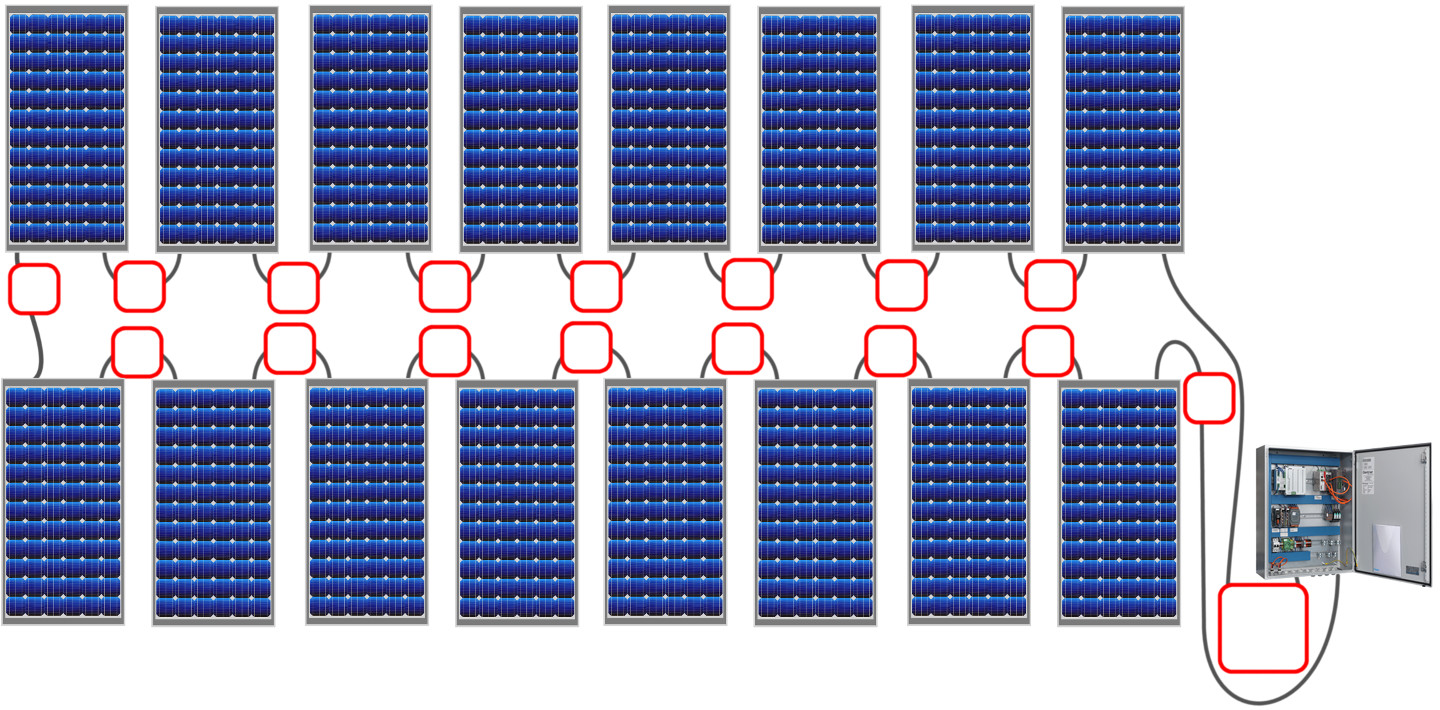
\includegraphics[width=\textwidth]{images/solar-facility/pvarray-ourSystem.jpeg}%
            };
            \node at (  3.5mm,-28.1mm) {S};
            \node at (13.75mm,-28mm) {S};
            \node at (28.75mm,-28mm) {S};
            \node at ( 43.5mm,-28mm) {S};
            \node at (58.25mm,-28mm) {S};
            \node at (72.75mm,-27.65mm) {S};
            \node at (87.75mm,-27.75mm) {S};
            \node at (102.25mm,-27.65mm) {S};

            \node at ( 13.5mm ,-34.4mm) {S};
            \node at ( 28.4mm ,-34.0mm) {S};
            \node at ( 43.45mm,-34.15mm) {S};
            \node at ( 57.2mm,-33.9mm) {S};
            \node at ( 71.75mm,-33.8mm) {S};
            \node at ( 86.65mm,-34.15mm) {S};
            \node at (102mm   ,-34.25mm) {S};

            \node at (117.7mm   ,-38.75mm) {S};

            \node at (122.75mm   ,-61.25mm) {\Huge M};
            %\node at (132mm,-55mm) {\small{GAK}};
            %\node at (120mm,0mm) {\small{Wechselrichter}};
            %\node at (55mm,-5mm) {\small{Modulstrang}};
        \end{scope}
    \end{tikzpicture}
    \caption[Modulstrang, \"Ubersichtsbild]{%
        Modulstrang mit je einem Sensor \textcolor{red}{S} pro Modul und einem
        \Master~\textcolor{red}{M} beim Generator-Anschlusskasten
    }
    \label{fig:pvarray:gak:inverter:ourSystem}
\end{figure}

Die    Installation   des    Master-Ger\"ates    erfolgt   im    zugeh\"origen
Schaltschrank. Das    Hutschienengeh\"ause    erm\"oglicht    eine    einfache
Installation in  bestehende oder  neue Schaltschr\"anke. Der Anschluss  an die
Energieversorgung  f\"ur das  Ger\"at selbst  wie auch  die Ankopplung  an die
DC-Leitungen  erfolgen im  Innern  des Schaltschrankes  und  werden von  einem
Elektroinstallateur ausgef\"uhrt.

Neben  dem   Klemmenanschluss  f\"ur   die  Energieversorgung  und   den  zwei
Relaisausg\"angen  f\"ur   externe  Alarmger\"ate   sieht  das   \Master~  die
Ankopplung der DC-Leitungen von bis zu drei Modulstr\"angen vor (einer gezeigt
in Abbildung \ref{fig:pvarray:gak:inverter:ourSystem}).

Ein  internes 2.5``  Touch-Display erm\"oglicht  eine einfache  Inbetriebnahme
und  eine benutzerfreundliche  Bedienung des  Systems. Alle Messresultate  der
Sensoren werden vom  \Master~ ausgewertet und dem Kunden  auf einer grafischen
Benutzeroberfl\"ache  dargestellt. Tritt ein  Fehler an  der Anlage  auf, wird
eine entsprechende Meldung auf dem Display angezeigt, die beiden Relais werden
bet\"atigt  und es  wird eine  Nachricht mittels  SMS versendet. Dadurch  wird
sichergestellt, dass der Kunde m\"oglichst schnell \"uber defekte PV-Module in
Kenntnis gesetzt wird.

\clearpage
Als Fehler werden folgende Ereignisse definiert:
\begin{itemize}
    \tightlist
    \item
        Eine defekte Zelle
    \item
        Eine dauerhaft verschmutzte Zelle
    \item
        Eine defekte Leitung
\end{itemize}

Kein Fehler soll in folgenden Situationen ausgel\"ost werden.
\begin{itemize}
    \tightlist
    \item
        Kurzzeitige Abschattungen (z.B. Vogel auf Zelle)
    \item
        Regelm\"assige Abschattungen,  die zu den  Umweltbedingungen geh\"oren
        (z.B. Baum, der t\"aglich abschattet)
    \item
        Nacht und schlechtes Wetter
    \item
        Anlage absichtlich ausser Betrieb genommen (z.B. Unterhaltsarbeiten)
\end{itemize}

F\"ur   die  Spannungsmessung   und   die   \"Ubertragung  der   Messresultate
sind  die   Sensoren  zust\"andig. Die   Installation  der   Sensoren  erfolgt
in  den   Anschlussdosen  auf  der  R\"uckseite   der  PV-Module. F\"ur  jedes
PV-Modul  ist   jeweils  ein   Sensor  zu   installieren,  wie   in  Abbildung
\ref{fig:pvarray:gak:inverter:ourSystem}  gezeigt. Eine zweiadrige  Verbindung
von der Sensorplatine  zu den Klemmen der Anschlussdose  ist zust\"andig f\"ur
die Energieversorgung  des Sensors. Die Einkopplung in  die DC-Leitung erfolgt
mit  einer  kleinen Induktionsspule,  durch  welche  die DC-Leitung  gef\"uhrt
wird. Dies erm\"oglicht das Kommunizieren mit dem \Master.


% ---------------------------------------------------------------------------- %
\section{Kommunikation \"uber DC-Leitung}
\label{sec:commDCLine}
% ---------------------------------------------------------------------------- %
\enlargethispage{2em}

Die Kommunikation  zwischen \Sensor~und \Master~\"uber die  DC-Leitung ist das
Herzst\"uck des Systems und das zu l\"osende Kernproblem des Projekts. Es sind
im Rahmen des  Projekts vier grunds\"atzliche Ans\"atze  untersucht worden, um
Daten  zwischen \Sensor~ und  \Master~  \"uber die  DC-Leitung  zu senden  und
empfangen.

\textbf{Frequency-shift keying}: Bei  der FSK (Frequenzumtastung  auf Deutsch)
wird  dem in  der Leitung  fliessenden Gleichstrom  ein (verh\"altnism\"assig)
kleines  Signal aufmoduliert,  welches  die  zu \"ubertragenden  Informationen
enth\"alt. Die Frequenz des aufmodulierten Anteils wird in diskreten Schritten
variiert und  jeweils einem  Symbol zugeordnet. Bei einer  bin\"aren Umsetzung
werden zwei Frequenzen benutzt; eine f\"ur \code{0} und eine f\"ur \code{1}.

\textbf{Amplitude-shift  keying}: Die  ASK (Amplitudenumtastung  auf  Deutsch)
benutzt statt verschiedenen Frequenzen unterschiedliche Amplituden, um Symbole
zu codieren.

\textbf{On-Off keying}: Bei  der OOK bedeuted die  Pr\"asenz einer Oszillation
auf  der  Leitung eine  \code{1},  die  Absenz von  Wechselstromanteilen  eine
logische  \code{0}. Eine   spezielle  Form   der  OOK,  welche   im  Abschnitt
\emph{\titleref{sec:simu:short}}  ab  Seite  \pageref{sec:simu:short}  genauer
untersucht  und  simuliert  wird,  benutzt  das  kontrollierte  Kurzschliessen
eines  PV-Moduls und  den  zugeh\"origen Spannungsabfall  zur Codierung  eines
Signals.

Abbildung   \ref{fig:modulation:concepts}   stellt    diese   vier   Varianten
vereinfacht dar,  zusammen mit dem  codierten Signal.  Aufgrund  der einfachen
Implementation haben  wird uns  f\"ur die Benutzung  einer OOK  mit Oszillator
entschieden.

\begin{figure}[h!tb]
    \centering
    %% Creator: Matplotlib, PGF backend
%%
%% To include the figure in your LaTeX document, write
%%   \input{<filename>.pgf}
%%
%% Make sure the required packages are loaded in your preamble
%%   \usepackage{pgf}
%%
%% Figures using additional raster images can only be included by \input if
%% they are in the same directory as the main LaTeX file. For loading figures
%% from other directories you can use the `import` package
%%   \usepackage{import}
%% and then include the figures with
%%   \import{<path to file>}{<filename>.pgf}
%%
%% Matplotlib used the following preamble
%%   \usepackage{fontspec}
%%   \setmainfont{Bitstream Vera Serif}
%%   \setsansfont{Bitstream Vera Sans}
%%   \setmonofont{Bitstream Vera Sans Mono}
%%
\begingroup%
\makeatletter%
\begin{pgfpicture}%
\pgfpathrectangle{\pgfpointorigin}{\pgfqpoint{5.100000in}{8.000000in}}%
\pgfusepath{use as bounding box, clip}%
\begin{pgfscope}%
\pgfsetbuttcap%
\pgfsetmiterjoin%
\pgfsetlinewidth{0.000000pt}%
\definecolor{currentstroke}{rgb}{0.000000,0.000000,0.000000}%
\pgfsetstrokecolor{currentstroke}%
\pgfsetstrokeopacity{0.000000}%
\pgfsetdash{}{0pt}%
\pgfpathmoveto{\pgfqpoint{0.000000in}{0.000000in}}%
\pgfpathlineto{\pgfqpoint{5.100000in}{0.000000in}}%
\pgfpathlineto{\pgfqpoint{5.100000in}{8.000000in}}%
\pgfpathlineto{\pgfqpoint{0.000000in}{8.000000in}}%
\pgfpathclose%
\pgfusepath{}%
\end{pgfscope}%
\begin{pgfscope}%
\pgfsetbuttcap%
\pgfsetmiterjoin%
\pgfsetlinewidth{0.000000pt}%
\definecolor{currentstroke}{rgb}{0.000000,0.000000,0.000000}%
\pgfsetstrokecolor{currentstroke}%
\pgfsetstrokeopacity{0.000000}%
\pgfsetdash{}{0pt}%
\pgfpathmoveto{\pgfqpoint{0.510000in}{6.541176in}}%
\pgfpathlineto{\pgfqpoint{4.845000in}{6.541176in}}%
\pgfpathlineto{\pgfqpoint{4.845000in}{7.600000in}}%
\pgfpathlineto{\pgfqpoint{0.510000in}{7.600000in}}%
\pgfpathclose%
\pgfusepath{}%
\end{pgfscope}%
\begin{pgfscope}%
\pgfpathrectangle{\pgfqpoint{0.510000in}{6.541176in}}{\pgfqpoint{4.335000in}{1.058824in}} %
\pgfusepath{clip}%
\pgfsetrectcap%
\pgfsetroundjoin%
\pgfsetlinewidth{0.501875pt}%
\definecolor{currentstroke}{rgb}{0.000000,0.000000,1.000000}%
\pgfsetstrokecolor{currentstroke}%
\pgfsetdash{}{0pt}%
\pgfpathmoveto{\pgfqpoint{0.510000in}{6.629412in}}%
\pgfpathlineto{\pgfqpoint{1.593750in}{6.629412in}}%
\pgfusepath{stroke}%
\end{pgfscope}%
\begin{pgfscope}%
\pgfpathrectangle{\pgfqpoint{0.510000in}{6.541176in}}{\pgfqpoint{4.335000in}{1.058824in}} %
\pgfusepath{clip}%
\pgfsetrectcap%
\pgfsetroundjoin%
\pgfsetlinewidth{0.501875pt}%
\definecolor{currentstroke}{rgb}{0.501961,0.501961,0.501961}%
\pgfsetstrokecolor{currentstroke}%
\pgfsetdash{}{0pt}%
\pgfpathmoveto{\pgfqpoint{1.593750in}{6.629412in}}%
\pgfpathlineto{\pgfqpoint{1.593750in}{7.511765in}}%
\pgfusepath{stroke}%
\end{pgfscope}%
\begin{pgfscope}%
\pgfpathrectangle{\pgfqpoint{0.510000in}{6.541176in}}{\pgfqpoint{4.335000in}{1.058824in}} %
\pgfusepath{clip}%
\pgfsetrectcap%
\pgfsetroundjoin%
\pgfsetlinewidth{0.501875pt}%
\definecolor{currentstroke}{rgb}{1.000000,0.000000,1.000000}%
\pgfsetstrokecolor{currentstroke}%
\pgfsetdash{}{0pt}%
\pgfpathmoveto{\pgfqpoint{1.593750in}{7.511765in}}%
\pgfpathlineto{\pgfqpoint{2.677500in}{7.511765in}}%
\pgfusepath{stroke}%
\end{pgfscope}%
\begin{pgfscope}%
\pgfpathrectangle{\pgfqpoint{0.510000in}{6.541176in}}{\pgfqpoint{4.335000in}{1.058824in}} %
\pgfusepath{clip}%
\pgfsetrectcap%
\pgfsetroundjoin%
\pgfsetlinewidth{0.501875pt}%
\definecolor{currentstroke}{rgb}{0.501961,0.501961,0.501961}%
\pgfsetstrokecolor{currentstroke}%
\pgfsetdash{}{0pt}%
\pgfpathmoveto{\pgfqpoint{2.677500in}{7.511765in}}%
\pgfpathlineto{\pgfqpoint{2.677500in}{6.629412in}}%
\pgfusepath{stroke}%
\end{pgfscope}%
\begin{pgfscope}%
\pgfpathrectangle{\pgfqpoint{0.510000in}{6.541176in}}{\pgfqpoint{4.335000in}{1.058824in}} %
\pgfusepath{clip}%
\pgfsetrectcap%
\pgfsetroundjoin%
\pgfsetlinewidth{0.501875pt}%
\definecolor{currentstroke}{rgb}{0.000000,0.000000,1.000000}%
\pgfsetstrokecolor{currentstroke}%
\pgfsetdash{}{0pt}%
\pgfpathmoveto{\pgfqpoint{2.677500in}{6.629412in}}%
\pgfpathlineto{\pgfqpoint{3.761250in}{6.629412in}}%
\pgfusepath{stroke}%
\end{pgfscope}%
\begin{pgfscope}%
\pgfpathrectangle{\pgfqpoint{0.510000in}{6.541176in}}{\pgfqpoint{4.335000in}{1.058824in}} %
\pgfusepath{clip}%
\pgfsetrectcap%
\pgfsetroundjoin%
\pgfsetlinewidth{0.501875pt}%
\definecolor{currentstroke}{rgb}{0.501961,0.501961,0.501961}%
\pgfsetstrokecolor{currentstroke}%
\pgfsetdash{}{0pt}%
\pgfpathmoveto{\pgfqpoint{3.761250in}{6.629412in}}%
\pgfpathlineto{\pgfqpoint{3.761250in}{7.511765in}}%
\pgfusepath{stroke}%
\end{pgfscope}%
\begin{pgfscope}%
\pgfpathrectangle{\pgfqpoint{0.510000in}{6.541176in}}{\pgfqpoint{4.335000in}{1.058824in}} %
\pgfusepath{clip}%
\pgfsetrectcap%
\pgfsetroundjoin%
\pgfsetlinewidth{0.501875pt}%
\definecolor{currentstroke}{rgb}{1.000000,0.000000,1.000000}%
\pgfsetstrokecolor{currentstroke}%
\pgfsetdash{}{0pt}%
\pgfpathmoveto{\pgfqpoint{3.761250in}{7.511765in}}%
\pgfpathlineto{\pgfqpoint{4.845000in}{7.511765in}}%
\pgfusepath{stroke}%
\end{pgfscope}%
\begin{pgfscope}%
\pgfsetrectcap%
\pgfsetmiterjoin%
\pgfsetlinewidth{0.501875pt}%
\definecolor{currentstroke}{rgb}{0.000000,0.000000,0.000000}%
\pgfsetstrokecolor{currentstroke}%
\pgfsetdash{}{0pt}%
\pgfpathmoveto{\pgfqpoint{0.510000in}{7.600000in}}%
\pgfpathlineto{\pgfqpoint{4.845000in}{7.600000in}}%
\pgfusepath{stroke}%
\end{pgfscope}%
\begin{pgfscope}%
\pgfsetrectcap%
\pgfsetmiterjoin%
\pgfsetlinewidth{0.501875pt}%
\definecolor{currentstroke}{rgb}{0.000000,0.000000,0.000000}%
\pgfsetstrokecolor{currentstroke}%
\pgfsetdash{}{0pt}%
\pgfpathmoveto{\pgfqpoint{0.510000in}{6.541176in}}%
\pgfpathlineto{\pgfqpoint{0.510000in}{7.600000in}}%
\pgfusepath{stroke}%
\end{pgfscope}%
\begin{pgfscope}%
\pgfsetrectcap%
\pgfsetmiterjoin%
\pgfsetlinewidth{0.501875pt}%
\definecolor{currentstroke}{rgb}{0.000000,0.000000,0.000000}%
\pgfsetstrokecolor{currentstroke}%
\pgfsetdash{}{0pt}%
\pgfpathmoveto{\pgfqpoint{0.510000in}{6.541176in}}%
\pgfpathlineto{\pgfqpoint{4.845000in}{6.541176in}}%
\pgfusepath{stroke}%
\end{pgfscope}%
\begin{pgfscope}%
\pgfsetrectcap%
\pgfsetmiterjoin%
\pgfsetlinewidth{0.501875pt}%
\definecolor{currentstroke}{rgb}{0.000000,0.000000,0.000000}%
\pgfsetstrokecolor{currentstroke}%
\pgfsetdash{}{0pt}%
\pgfpathmoveto{\pgfqpoint{4.845000in}{6.541176in}}%
\pgfpathlineto{\pgfqpoint{4.845000in}{7.600000in}}%
\pgfusepath{stroke}%
\end{pgfscope}%
\begin{pgfscope}%
\pgftext[x=2.677500in,y=6.471732in,,top]{\rmfamily\fontsize{9.000000}{10.800000}\selectfont Zeit}%
\end{pgfscope}%
\begin{pgfscope}%
\pgfsetbuttcap%
\pgfsetroundjoin%
\definecolor{currentfill}{rgb}{0.000000,0.000000,0.000000}%
\pgfsetfillcolor{currentfill}%
\pgfsetlinewidth{0.501875pt}%
\definecolor{currentstroke}{rgb}{0.000000,0.000000,0.000000}%
\pgfsetstrokecolor{currentstroke}%
\pgfsetdash{}{0pt}%
\pgfsys@defobject{currentmarker}{\pgfqpoint{0.000000in}{0.000000in}}{\pgfqpoint{0.055556in}{0.000000in}}{%
\pgfpathmoveto{\pgfqpoint{0.000000in}{0.000000in}}%
\pgfpathlineto{\pgfqpoint{0.055556in}{0.000000in}}%
\pgfusepath{stroke,fill}%
}%
\begin{pgfscope}%
\pgfsys@transformshift{0.510000in}{6.629412in}%
\pgfsys@useobject{currentmarker}{}%
\end{pgfscope}%
\end{pgfscope}%
\begin{pgfscope}%
\pgfsetbuttcap%
\pgfsetroundjoin%
\definecolor{currentfill}{rgb}{0.000000,0.000000,0.000000}%
\pgfsetfillcolor{currentfill}%
\pgfsetlinewidth{0.501875pt}%
\definecolor{currentstroke}{rgb}{0.000000,0.000000,0.000000}%
\pgfsetstrokecolor{currentstroke}%
\pgfsetdash{}{0pt}%
\pgfsys@defobject{currentmarker}{\pgfqpoint{-0.055556in}{0.000000in}}{\pgfqpoint{0.000000in}{0.000000in}}{%
\pgfpathmoveto{\pgfqpoint{0.000000in}{0.000000in}}%
\pgfpathlineto{\pgfqpoint{-0.055556in}{0.000000in}}%
\pgfusepath{stroke,fill}%
}%
\begin{pgfscope}%
\pgfsys@transformshift{4.845000in}{6.629412in}%
\pgfsys@useobject{currentmarker}{}%
\end{pgfscope}%
\end{pgfscope}%
\begin{pgfscope}%
\pgftext[x=0.454444in,y=6.629412in,right,]{\rmfamily\fontsize{9.000000}{10.800000}\selectfont \(\displaystyle 0\)}%
\end{pgfscope}%
\begin{pgfscope}%
\pgfsetbuttcap%
\pgfsetroundjoin%
\definecolor{currentfill}{rgb}{0.000000,0.000000,0.000000}%
\pgfsetfillcolor{currentfill}%
\pgfsetlinewidth{0.501875pt}%
\definecolor{currentstroke}{rgb}{0.000000,0.000000,0.000000}%
\pgfsetstrokecolor{currentstroke}%
\pgfsetdash{}{0pt}%
\pgfsys@defobject{currentmarker}{\pgfqpoint{0.000000in}{0.000000in}}{\pgfqpoint{0.055556in}{0.000000in}}{%
\pgfpathmoveto{\pgfqpoint{0.000000in}{0.000000in}}%
\pgfpathlineto{\pgfqpoint{0.055556in}{0.000000in}}%
\pgfusepath{stroke,fill}%
}%
\begin{pgfscope}%
\pgfsys@transformshift{0.510000in}{7.511765in}%
\pgfsys@useobject{currentmarker}{}%
\end{pgfscope}%
\end{pgfscope}%
\begin{pgfscope}%
\pgfsetbuttcap%
\pgfsetroundjoin%
\definecolor{currentfill}{rgb}{0.000000,0.000000,0.000000}%
\pgfsetfillcolor{currentfill}%
\pgfsetlinewidth{0.501875pt}%
\definecolor{currentstroke}{rgb}{0.000000,0.000000,0.000000}%
\pgfsetstrokecolor{currentstroke}%
\pgfsetdash{}{0pt}%
\pgfsys@defobject{currentmarker}{\pgfqpoint{-0.055556in}{0.000000in}}{\pgfqpoint{0.000000in}{0.000000in}}{%
\pgfpathmoveto{\pgfqpoint{0.000000in}{0.000000in}}%
\pgfpathlineto{\pgfqpoint{-0.055556in}{0.000000in}}%
\pgfusepath{stroke,fill}%
}%
\begin{pgfscope}%
\pgfsys@transformshift{4.845000in}{7.511765in}%
\pgfsys@useobject{currentmarker}{}%
\end{pgfscope}%
\end{pgfscope}%
\begin{pgfscope}%
\pgftext[x=0.454444in,y=7.511765in,right,]{\rmfamily\fontsize{9.000000}{10.800000}\selectfont \(\displaystyle 1\)}%
\end{pgfscope}%
\begin{pgfscope}%
\pgftext[x=0.320764in,y=7.070588in,,bottom,rotate=90.000000]{\rmfamily\fontsize{9.000000}{10.800000}\selectfont Symbol}%
\end{pgfscope}%
\begin{pgfscope}%
\pgftext[x=2.677500in,y=7.669444in,,base]{\rmfamily\fontsize{11.000000}{13.200000}\selectfont Daten}%
\end{pgfscope}%
\begin{pgfscope}%
\pgfsetbuttcap%
\pgfsetmiterjoin%
\pgfsetlinewidth{0.000000pt}%
\definecolor{currentstroke}{rgb}{0.000000,0.000000,0.000000}%
\pgfsetstrokecolor{currentstroke}%
\pgfsetstrokeopacity{0.000000}%
\pgfsetdash{}{0pt}%
\pgfpathmoveto{\pgfqpoint{0.510000in}{5.005882in}}%
\pgfpathlineto{\pgfqpoint{4.845000in}{5.005882in}}%
\pgfpathlineto{\pgfqpoint{4.845000in}{6.064706in}}%
\pgfpathlineto{\pgfqpoint{0.510000in}{6.064706in}}%
\pgfpathclose%
\pgfusepath{}%
\end{pgfscope}%
\begin{pgfscope}%
\pgfpathrectangle{\pgfqpoint{0.510000in}{5.005882in}}{\pgfqpoint{4.335000in}{1.058824in}} %
\pgfusepath{clip}%
\pgfsetrectcap%
\pgfsetroundjoin%
\pgfsetlinewidth{0.501875pt}%
\definecolor{currentstroke}{rgb}{0.000000,0.000000,1.000000}%
\pgfsetstrokecolor{currentstroke}%
\pgfsetdash{}{0pt}%
\pgfpathmoveto{\pgfqpoint{0.510000in}{5.054011in}}%
\pgfpathlineto{\pgfqpoint{0.515424in}{5.054962in}}%
\pgfpathlineto{\pgfqpoint{0.521933in}{5.058611in}}%
\pgfpathlineto{\pgfqpoint{0.528442in}{5.064973in}}%
\pgfpathlineto{\pgfqpoint{0.536036in}{5.075777in}}%
\pgfpathlineto{\pgfqpoint{0.544715in}{5.092478in}}%
\pgfpathlineto{\pgfqpoint{0.554478in}{5.116611in}}%
\pgfpathlineto{\pgfqpoint{0.565327in}{5.149698in}}%
\pgfpathlineto{\pgfqpoint{0.578345in}{5.197392in}}%
\pgfpathlineto{\pgfqpoint{0.593532in}{5.262661in}}%
\pgfpathlineto{\pgfqpoint{0.611974in}{5.353039in}}%
\pgfpathlineto{\pgfqpoint{0.636926in}{5.487696in}}%
\pgfpathlineto{\pgfqpoint{0.683574in}{5.741091in}}%
\pgfpathlineto{\pgfqpoint{0.702016in}{5.828731in}}%
\pgfpathlineto{\pgfqpoint{0.717203in}{5.891027in}}%
\pgfpathlineto{\pgfqpoint{0.730221in}{5.935729in}}%
\pgfpathlineto{\pgfqpoint{0.741070in}{5.966062in}}%
\pgfpathlineto{\pgfqpoint{0.750833in}{5.987553in}}%
\pgfpathlineto{\pgfqpoint{0.759512in}{6.001801in}}%
\pgfpathlineto{\pgfqpoint{0.767106in}{6.010401in}}%
\pgfpathlineto{\pgfqpoint{0.773615in}{6.014844in}}%
\pgfpathlineto{\pgfqpoint{0.780124in}{6.016556in}}%
\pgfpathlineto{\pgfqpoint{0.785548in}{6.015890in}}%
\pgfpathlineto{\pgfqpoint{0.792057in}{6.012583in}}%
\pgfpathlineto{\pgfqpoint{0.798566in}{6.006558in}}%
\pgfpathlineto{\pgfqpoint{0.806160in}{5.996141in}}%
\pgfpathlineto{\pgfqpoint{0.814839in}{5.979870in}}%
\pgfpathlineto{\pgfqpoint{0.824602in}{5.956197in}}%
\pgfpathlineto{\pgfqpoint{0.835450in}{5.923590in}}%
\pgfpathlineto{\pgfqpoint{0.847384in}{5.880658in}}%
\pgfpathlineto{\pgfqpoint{0.861486in}{5.821481in}}%
\pgfpathlineto{\pgfqpoint{0.878844in}{5.738350in}}%
\pgfpathlineto{\pgfqpoint{0.901625in}{5.617377in}}%
\pgfpathlineto{\pgfqpoint{0.959122in}{5.306544in}}%
\pgfpathlineto{\pgfqpoint{0.976479in}{5.226511in}}%
\pgfpathlineto{\pgfqpoint{0.991667in}{5.166610in}}%
\pgfpathlineto{\pgfqpoint{1.004685in}{5.124282in}}%
\pgfpathlineto{\pgfqpoint{1.015533in}{5.096114in}}%
\pgfpathlineto{\pgfqpoint{1.025297in}{5.076686in}}%
\pgfpathlineto{\pgfqpoint{1.033975in}{5.064340in}}%
\pgfpathlineto{\pgfqpoint{1.041569in}{5.057443in}}%
\pgfpathlineto{\pgfqpoint{1.048078in}{5.054477in}}%
\pgfpathlineto{\pgfqpoint{1.053502in}{5.054096in}}%
\pgfpathlineto{\pgfqpoint{1.058926in}{5.055619in}}%
\pgfpathlineto{\pgfqpoint{1.065435in}{5.059948in}}%
\pgfpathlineto{\pgfqpoint{1.071944in}{5.066984in}}%
\pgfpathlineto{\pgfqpoint{1.079538in}{5.078559in}}%
\pgfpathlineto{\pgfqpoint{1.088217in}{5.096114in}}%
\pgfpathlineto{\pgfqpoint{1.097980in}{5.121164in}}%
\pgfpathlineto{\pgfqpoint{1.108829in}{5.155200in}}%
\pgfpathlineto{\pgfqpoint{1.121847in}{5.203918in}}%
\pgfpathlineto{\pgfqpoint{1.137035in}{5.270193in}}%
\pgfpathlineto{\pgfqpoint{1.155477in}{5.361476in}}%
\pgfpathlineto{\pgfqpoint{1.182598in}{5.508821in}}%
\pgfpathlineto{\pgfqpoint{1.223821in}{5.732846in}}%
\pgfpathlineto{\pgfqpoint{1.243348in}{5.826326in}}%
\pgfpathlineto{\pgfqpoint{1.258536in}{5.888981in}}%
\pgfpathlineto{\pgfqpoint{1.271554in}{5.934042in}}%
\pgfpathlineto{\pgfqpoint{1.283487in}{5.967403in}}%
\pgfpathlineto{\pgfqpoint{1.293251in}{5.988579in}}%
\pgfpathlineto{\pgfqpoint{1.301929in}{6.002537in}}%
\pgfpathlineto{\pgfqpoint{1.309523in}{6.010875in}}%
\pgfpathlineto{\pgfqpoint{1.316032in}{6.015091in}}%
\pgfpathlineto{\pgfqpoint{1.322541in}{6.016575in}}%
\pgfpathlineto{\pgfqpoint{1.327965in}{6.015719in}}%
\pgfpathlineto{\pgfqpoint{1.334474in}{6.012184in}}%
\pgfpathlineto{\pgfqpoint{1.340983in}{6.005934in}}%
\pgfpathlineto{\pgfqpoint{1.348577in}{5.995259in}}%
\pgfpathlineto{\pgfqpoint{1.357256in}{5.978701in}}%
\pgfpathlineto{\pgfqpoint{1.367020in}{5.954721in}}%
\pgfpathlineto{\pgfqpoint{1.377868in}{5.921794in}}%
\pgfpathlineto{\pgfqpoint{1.390886in}{5.874272in}}%
\pgfpathlineto{\pgfqpoint{1.406074in}{5.809173in}}%
\pgfpathlineto{\pgfqpoint{1.424516in}{5.718949in}}%
\pgfpathlineto{\pgfqpoint{1.449467in}{5.584398in}}%
\pgfpathlineto{\pgfqpoint{1.497200in}{5.325402in}}%
\pgfpathlineto{\pgfqpoint{1.515642in}{5.238271in}}%
\pgfpathlineto{\pgfqpoint{1.530830in}{5.176519in}}%
\pgfpathlineto{\pgfqpoint{1.543848in}{5.132358in}}%
\pgfpathlineto{\pgfqpoint{1.554696in}{5.102521in}}%
\pgfpathlineto{\pgfqpoint{1.564459in}{5.081503in}}%
\pgfpathlineto{\pgfqpoint{1.573138in}{5.067691in}}%
\pgfpathlineto{\pgfqpoint{1.580732in}{5.059483in}}%
\pgfpathlineto{\pgfqpoint{1.587241in}{5.055381in}}%
\pgfpathlineto{\pgfqpoint{1.593750in}{5.054011in}}%
\pgfpathlineto{\pgfqpoint{1.593750in}{5.054011in}}%
\pgfusepath{stroke}%
\end{pgfscope}%
\begin{pgfscope}%
\pgfpathrectangle{\pgfqpoint{0.510000in}{5.005882in}}{\pgfqpoint{4.335000in}{1.058824in}} %
\pgfusepath{clip}%
\pgfsetrectcap%
\pgfsetroundjoin%
\pgfsetlinewidth{0.501875pt}%
\definecolor{currentstroke}{rgb}{1.000000,0.000000,1.000000}%
\pgfsetstrokecolor{currentstroke}%
\pgfsetdash{}{0pt}%
\pgfpathmoveto{\pgfqpoint{1.593750in}{5.054011in}}%
\pgfpathlineto{\pgfqpoint{1.595920in}{5.055381in}}%
\pgfpathlineto{\pgfqpoint{1.599174in}{5.062553in}}%
\pgfpathlineto{\pgfqpoint{1.603514in}{5.081503in}}%
\pgfpathlineto{\pgfqpoint{1.608938in}{5.119630in}}%
\pgfpathlineto{\pgfqpoint{1.615447in}{5.184702in}}%
\pgfpathlineto{\pgfqpoint{1.624125in}{5.298595in}}%
\pgfpathlineto{\pgfqpoint{1.637143in}{5.505799in}}%
\pgfpathlineto{\pgfqpoint{1.656670in}{5.814130in}}%
\pgfpathlineto{\pgfqpoint{1.665349in}{5.918156in}}%
\pgfpathlineto{\pgfqpoint{1.671858in}{5.973853in}}%
\pgfpathlineto{\pgfqpoint{1.677282in}{6.003253in}}%
\pgfpathlineto{\pgfqpoint{1.681622in}{6.014844in}}%
\pgfpathlineto{\pgfqpoint{1.683791in}{6.016556in}}%
\pgfpathlineto{\pgfqpoint{1.685961in}{6.015528in}}%
\pgfpathlineto{\pgfqpoint{1.688131in}{6.011766in}}%
\pgfpathlineto{\pgfqpoint{1.691385in}{6.001048in}}%
\pgfpathlineto{\pgfqpoint{1.695724in}{5.977515in}}%
\pgfpathlineto{\pgfqpoint{1.701149in}{5.934042in}}%
\pgfpathlineto{\pgfqpoint{1.707658in}{5.863363in}}%
\pgfpathlineto{\pgfqpoint{1.716336in}{5.743823in}}%
\pgfpathlineto{\pgfqpoint{1.731524in}{5.496741in}}%
\pgfpathlineto{\pgfqpoint{1.746712in}{5.260172in}}%
\pgfpathlineto{\pgfqpoint{1.755390in}{5.155200in}}%
\pgfpathlineto{\pgfqpoint{1.761899in}{5.098625in}}%
\pgfpathlineto{\pgfqpoint{1.767324in}{5.068417in}}%
\pgfpathlineto{\pgfqpoint{1.771663in}{5.056151in}}%
\pgfpathlineto{\pgfqpoint{1.773833in}{5.054096in}}%
\pgfpathlineto{\pgfqpoint{1.776002in}{5.054782in}}%
\pgfpathlineto{\pgfqpoint{1.778172in}{5.058203in}}%
\pgfpathlineto{\pgfqpoint{1.781426in}{5.068417in}}%
\pgfpathlineto{\pgfqpoint{1.785766in}{5.091301in}}%
\pgfpathlineto{\pgfqpoint{1.791190in}{5.134021in}}%
\pgfpathlineto{\pgfqpoint{1.797699in}{5.203918in}}%
\pgfpathlineto{\pgfqpoint{1.806378in}{5.322682in}}%
\pgfpathlineto{\pgfqpoint{1.821565in}{5.569320in}}%
\pgfpathlineto{\pgfqpoint{1.836753in}{5.806679in}}%
\pgfpathlineto{\pgfqpoint{1.845432in}{5.912586in}}%
\pgfpathlineto{\pgfqpoint{1.851941in}{5.970035in}}%
\pgfpathlineto{\pgfqpoint{1.857365in}{6.001048in}}%
\pgfpathlineto{\pgfqpoint{1.861704in}{6.013988in}}%
\pgfpathlineto{\pgfqpoint{1.863874in}{6.016385in}}%
\pgfpathlineto{\pgfqpoint{1.866044in}{6.016042in}}%
\pgfpathlineto{\pgfqpoint{1.868213in}{6.012962in}}%
\pgfpathlineto{\pgfqpoint{1.871468in}{6.003253in}}%
\pgfpathlineto{\pgfqpoint{1.875807in}{5.981020in}}%
\pgfpathlineto{\pgfqpoint{1.881231in}{5.939056in}}%
\pgfpathlineto{\pgfqpoint{1.887740in}{5.869948in}}%
\pgfpathlineto{\pgfqpoint{1.896419in}{5.751970in}}%
\pgfpathlineto{\pgfqpoint{1.910522in}{5.523944in}}%
\pgfpathlineto{\pgfqpoint{1.926794in}{5.267671in}}%
\pgfpathlineto{\pgfqpoint{1.935473in}{5.160838in}}%
\pgfpathlineto{\pgfqpoint{1.941982in}{5.102521in}}%
\pgfpathlineto{\pgfqpoint{1.947406in}{5.070705in}}%
\pgfpathlineto{\pgfqpoint{1.951745in}{5.057092in}}%
\pgfpathlineto{\pgfqpoint{1.955000in}{5.054011in}}%
\pgfpathlineto{\pgfqpoint{1.957170in}{5.055381in}}%
\pgfpathlineto{\pgfqpoint{1.960424in}{5.062553in}}%
\pgfpathlineto{\pgfqpoint{1.964764in}{5.081503in}}%
\pgfpathlineto{\pgfqpoint{1.970188in}{5.119630in}}%
\pgfpathlineto{\pgfqpoint{1.976697in}{5.184702in}}%
\pgfpathlineto{\pgfqpoint{1.985375in}{5.298595in}}%
\pgfpathlineto{\pgfqpoint{1.998393in}{5.505799in}}%
\pgfpathlineto{\pgfqpoint{2.017920in}{5.814130in}}%
\pgfpathlineto{\pgfqpoint{2.026599in}{5.918156in}}%
\pgfpathlineto{\pgfqpoint{2.033108in}{5.973853in}}%
\pgfpathlineto{\pgfqpoint{2.038532in}{6.003253in}}%
\pgfpathlineto{\pgfqpoint{2.042872in}{6.014844in}}%
\pgfpathlineto{\pgfqpoint{2.045041in}{6.016556in}}%
\pgfpathlineto{\pgfqpoint{2.047211in}{6.015528in}}%
\pgfpathlineto{\pgfqpoint{2.049381in}{6.011766in}}%
\pgfpathlineto{\pgfqpoint{2.052635in}{6.001048in}}%
\pgfpathlineto{\pgfqpoint{2.056974in}{5.977515in}}%
\pgfpathlineto{\pgfqpoint{2.062399in}{5.934042in}}%
\pgfpathlineto{\pgfqpoint{2.068908in}{5.863363in}}%
\pgfpathlineto{\pgfqpoint{2.077586in}{5.743823in}}%
\pgfpathlineto{\pgfqpoint{2.092774in}{5.496741in}}%
\pgfpathlineto{\pgfqpoint{2.107962in}{5.260172in}}%
\pgfpathlineto{\pgfqpoint{2.116640in}{5.155200in}}%
\pgfpathlineto{\pgfqpoint{2.123149in}{5.098625in}}%
\pgfpathlineto{\pgfqpoint{2.128574in}{5.068417in}}%
\pgfpathlineto{\pgfqpoint{2.132913in}{5.056151in}}%
\pgfpathlineto{\pgfqpoint{2.135083in}{5.054096in}}%
\pgfpathlineto{\pgfqpoint{2.137252in}{5.054782in}}%
\pgfpathlineto{\pgfqpoint{2.139422in}{5.058203in}}%
\pgfpathlineto{\pgfqpoint{2.142676in}{5.068417in}}%
\pgfpathlineto{\pgfqpoint{2.147016in}{5.091301in}}%
\pgfpathlineto{\pgfqpoint{2.152440in}{5.134021in}}%
\pgfpathlineto{\pgfqpoint{2.158949in}{5.203918in}}%
\pgfpathlineto{\pgfqpoint{2.167628in}{5.322682in}}%
\pgfpathlineto{\pgfqpoint{2.182815in}{5.569320in}}%
\pgfpathlineto{\pgfqpoint{2.198003in}{5.806679in}}%
\pgfpathlineto{\pgfqpoint{2.206682in}{5.912586in}}%
\pgfpathlineto{\pgfqpoint{2.213191in}{5.970035in}}%
\pgfpathlineto{\pgfqpoint{2.218615in}{6.001048in}}%
\pgfpathlineto{\pgfqpoint{2.222954in}{6.013988in}}%
\pgfpathlineto{\pgfqpoint{2.225124in}{6.016385in}}%
\pgfpathlineto{\pgfqpoint{2.227294in}{6.016042in}}%
\pgfpathlineto{\pgfqpoint{2.229463in}{6.012962in}}%
\pgfpathlineto{\pgfqpoint{2.232718in}{6.003253in}}%
\pgfpathlineto{\pgfqpoint{2.237057in}{5.981020in}}%
\pgfpathlineto{\pgfqpoint{2.242481in}{5.939056in}}%
\pgfpathlineto{\pgfqpoint{2.248990in}{5.869948in}}%
\pgfpathlineto{\pgfqpoint{2.257669in}{5.751970in}}%
\pgfpathlineto{\pgfqpoint{2.271772in}{5.523944in}}%
\pgfpathlineto{\pgfqpoint{2.288044in}{5.267671in}}%
\pgfpathlineto{\pgfqpoint{2.296723in}{5.160838in}}%
\pgfpathlineto{\pgfqpoint{2.303232in}{5.102521in}}%
\pgfpathlineto{\pgfqpoint{2.308656in}{5.070705in}}%
\pgfpathlineto{\pgfqpoint{2.312995in}{5.057092in}}%
\pgfpathlineto{\pgfqpoint{2.316250in}{5.054011in}}%
\pgfpathlineto{\pgfqpoint{2.318420in}{5.055381in}}%
\pgfpathlineto{\pgfqpoint{2.321674in}{5.062553in}}%
\pgfpathlineto{\pgfqpoint{2.326014in}{5.081503in}}%
\pgfpathlineto{\pgfqpoint{2.331438in}{5.119630in}}%
\pgfpathlineto{\pgfqpoint{2.337947in}{5.184702in}}%
\pgfpathlineto{\pgfqpoint{2.346625in}{5.298595in}}%
\pgfpathlineto{\pgfqpoint{2.359643in}{5.505799in}}%
\pgfpathlineto{\pgfqpoint{2.379170in}{5.814130in}}%
\pgfpathlineto{\pgfqpoint{2.387849in}{5.918156in}}%
\pgfpathlineto{\pgfqpoint{2.394358in}{5.973853in}}%
\pgfpathlineto{\pgfqpoint{2.399782in}{6.003253in}}%
\pgfpathlineto{\pgfqpoint{2.404122in}{6.014844in}}%
\pgfpathlineto{\pgfqpoint{2.406291in}{6.016556in}}%
\pgfpathlineto{\pgfqpoint{2.408461in}{6.015528in}}%
\pgfpathlineto{\pgfqpoint{2.410631in}{6.011766in}}%
\pgfpathlineto{\pgfqpoint{2.413885in}{6.001048in}}%
\pgfpathlineto{\pgfqpoint{2.418224in}{5.977515in}}%
\pgfpathlineto{\pgfqpoint{2.423649in}{5.934042in}}%
\pgfpathlineto{\pgfqpoint{2.430158in}{5.863363in}}%
\pgfpathlineto{\pgfqpoint{2.438836in}{5.743823in}}%
\pgfpathlineto{\pgfqpoint{2.454024in}{5.496741in}}%
\pgfpathlineto{\pgfqpoint{2.469212in}{5.260172in}}%
\pgfpathlineto{\pgfqpoint{2.477890in}{5.155200in}}%
\pgfpathlineto{\pgfqpoint{2.484399in}{5.098625in}}%
\pgfpathlineto{\pgfqpoint{2.489824in}{5.068417in}}%
\pgfpathlineto{\pgfqpoint{2.494163in}{5.056151in}}%
\pgfpathlineto{\pgfqpoint{2.496333in}{5.054096in}}%
\pgfpathlineto{\pgfqpoint{2.498502in}{5.054782in}}%
\pgfpathlineto{\pgfqpoint{2.500672in}{5.058203in}}%
\pgfpathlineto{\pgfqpoint{2.503926in}{5.068417in}}%
\pgfpathlineto{\pgfqpoint{2.508266in}{5.091301in}}%
\pgfpathlineto{\pgfqpoint{2.513690in}{5.134021in}}%
\pgfpathlineto{\pgfqpoint{2.520199in}{5.203918in}}%
\pgfpathlineto{\pgfqpoint{2.528878in}{5.322682in}}%
\pgfpathlineto{\pgfqpoint{2.544065in}{5.569320in}}%
\pgfpathlineto{\pgfqpoint{2.559253in}{5.806679in}}%
\pgfpathlineto{\pgfqpoint{2.567932in}{5.912586in}}%
\pgfpathlineto{\pgfqpoint{2.574441in}{5.970035in}}%
\pgfpathlineto{\pgfqpoint{2.579865in}{6.001048in}}%
\pgfpathlineto{\pgfqpoint{2.584204in}{6.013988in}}%
\pgfpathlineto{\pgfqpoint{2.586374in}{6.016385in}}%
\pgfpathlineto{\pgfqpoint{2.588544in}{6.016042in}}%
\pgfpathlineto{\pgfqpoint{2.590713in}{6.012962in}}%
\pgfpathlineto{\pgfqpoint{2.593968in}{6.003253in}}%
\pgfpathlineto{\pgfqpoint{2.598307in}{5.981020in}}%
\pgfpathlineto{\pgfqpoint{2.603731in}{5.939056in}}%
\pgfpathlineto{\pgfqpoint{2.610240in}{5.869948in}}%
\pgfpathlineto{\pgfqpoint{2.618919in}{5.751970in}}%
\pgfpathlineto{\pgfqpoint{2.633022in}{5.523944in}}%
\pgfpathlineto{\pgfqpoint{2.649294in}{5.267671in}}%
\pgfpathlineto{\pgfqpoint{2.657973in}{5.160838in}}%
\pgfpathlineto{\pgfqpoint{2.664482in}{5.102521in}}%
\pgfpathlineto{\pgfqpoint{2.669906in}{5.070705in}}%
\pgfpathlineto{\pgfqpoint{2.674245in}{5.057092in}}%
\pgfpathlineto{\pgfqpoint{2.677500in}{5.054011in}}%
\pgfpathlineto{\pgfqpoint{2.677500in}{5.054011in}}%
\pgfusepath{stroke}%
\end{pgfscope}%
\begin{pgfscope}%
\pgfpathrectangle{\pgfqpoint{0.510000in}{5.005882in}}{\pgfqpoint{4.335000in}{1.058824in}} %
\pgfusepath{clip}%
\pgfsetrectcap%
\pgfsetroundjoin%
\pgfsetlinewidth{0.501875pt}%
\definecolor{currentstroke}{rgb}{0.000000,0.000000,1.000000}%
\pgfsetstrokecolor{currentstroke}%
\pgfsetdash{}{0pt}%
\pgfpathmoveto{\pgfqpoint{2.677500in}{5.054011in}}%
\pgfpathlineto{\pgfqpoint{2.682924in}{5.054962in}}%
\pgfpathlineto{\pgfqpoint{2.689433in}{5.058611in}}%
\pgfpathlineto{\pgfqpoint{2.695942in}{5.064973in}}%
\pgfpathlineto{\pgfqpoint{2.703536in}{5.075777in}}%
\pgfpathlineto{\pgfqpoint{2.712215in}{5.092478in}}%
\pgfpathlineto{\pgfqpoint{2.721978in}{5.116611in}}%
\pgfpathlineto{\pgfqpoint{2.732827in}{5.149698in}}%
\pgfpathlineto{\pgfqpoint{2.745845in}{5.197392in}}%
\pgfpathlineto{\pgfqpoint{2.761032in}{5.262661in}}%
\pgfpathlineto{\pgfqpoint{2.779474in}{5.353039in}}%
\pgfpathlineto{\pgfqpoint{2.804426in}{5.487696in}}%
\pgfpathlineto{\pgfqpoint{2.851074in}{5.741091in}}%
\pgfpathlineto{\pgfqpoint{2.869516in}{5.828731in}}%
\pgfpathlineto{\pgfqpoint{2.884703in}{5.891027in}}%
\pgfpathlineto{\pgfqpoint{2.897721in}{5.935729in}}%
\pgfpathlineto{\pgfqpoint{2.908570in}{5.966062in}}%
\pgfpathlineto{\pgfqpoint{2.918333in}{5.987553in}}%
\pgfpathlineto{\pgfqpoint{2.927012in}{6.001801in}}%
\pgfpathlineto{\pgfqpoint{2.934606in}{6.010401in}}%
\pgfpathlineto{\pgfqpoint{2.941115in}{6.014844in}}%
\pgfpathlineto{\pgfqpoint{2.947624in}{6.016556in}}%
\pgfpathlineto{\pgfqpoint{2.953048in}{6.015890in}}%
\pgfpathlineto{\pgfqpoint{2.959557in}{6.012583in}}%
\pgfpathlineto{\pgfqpoint{2.966066in}{6.006558in}}%
\pgfpathlineto{\pgfqpoint{2.973660in}{5.996141in}}%
\pgfpathlineto{\pgfqpoint{2.982339in}{5.979870in}}%
\pgfpathlineto{\pgfqpoint{2.992102in}{5.956197in}}%
\pgfpathlineto{\pgfqpoint{3.002950in}{5.923590in}}%
\pgfpathlineto{\pgfqpoint{3.014884in}{5.880658in}}%
\pgfpathlineto{\pgfqpoint{3.028986in}{5.821481in}}%
\pgfpathlineto{\pgfqpoint{3.046344in}{5.738350in}}%
\pgfpathlineto{\pgfqpoint{3.069125in}{5.617377in}}%
\pgfpathlineto{\pgfqpoint{3.126622in}{5.306544in}}%
\pgfpathlineto{\pgfqpoint{3.143979in}{5.226511in}}%
\pgfpathlineto{\pgfqpoint{3.159167in}{5.166610in}}%
\pgfpathlineto{\pgfqpoint{3.172185in}{5.124282in}}%
\pgfpathlineto{\pgfqpoint{3.183033in}{5.096114in}}%
\pgfpathlineto{\pgfqpoint{3.192797in}{5.076686in}}%
\pgfpathlineto{\pgfqpoint{3.201475in}{5.064340in}}%
\pgfpathlineto{\pgfqpoint{3.209069in}{5.057443in}}%
\pgfpathlineto{\pgfqpoint{3.215578in}{5.054477in}}%
\pgfpathlineto{\pgfqpoint{3.221002in}{5.054096in}}%
\pgfpathlineto{\pgfqpoint{3.226426in}{5.055619in}}%
\pgfpathlineto{\pgfqpoint{3.232935in}{5.059948in}}%
\pgfpathlineto{\pgfqpoint{3.239444in}{5.066984in}}%
\pgfpathlineto{\pgfqpoint{3.247038in}{5.078559in}}%
\pgfpathlineto{\pgfqpoint{3.255717in}{5.096114in}}%
\pgfpathlineto{\pgfqpoint{3.265480in}{5.121164in}}%
\pgfpathlineto{\pgfqpoint{3.276329in}{5.155200in}}%
\pgfpathlineto{\pgfqpoint{3.289347in}{5.203918in}}%
\pgfpathlineto{\pgfqpoint{3.304535in}{5.270193in}}%
\pgfpathlineto{\pgfqpoint{3.322977in}{5.361476in}}%
\pgfpathlineto{\pgfqpoint{3.350098in}{5.508821in}}%
\pgfpathlineto{\pgfqpoint{3.391321in}{5.732846in}}%
\pgfpathlineto{\pgfqpoint{3.410848in}{5.826326in}}%
\pgfpathlineto{\pgfqpoint{3.426036in}{5.888981in}}%
\pgfpathlineto{\pgfqpoint{3.439054in}{5.934042in}}%
\pgfpathlineto{\pgfqpoint{3.450987in}{5.967403in}}%
\pgfpathlineto{\pgfqpoint{3.460751in}{5.988579in}}%
\pgfpathlineto{\pgfqpoint{3.469429in}{6.002537in}}%
\pgfpathlineto{\pgfqpoint{3.477023in}{6.010875in}}%
\pgfpathlineto{\pgfqpoint{3.483532in}{6.015091in}}%
\pgfpathlineto{\pgfqpoint{3.490041in}{6.016575in}}%
\pgfpathlineto{\pgfqpoint{3.495465in}{6.015719in}}%
\pgfpathlineto{\pgfqpoint{3.501974in}{6.012184in}}%
\pgfpathlineto{\pgfqpoint{3.508483in}{6.005934in}}%
\pgfpathlineto{\pgfqpoint{3.516077in}{5.995259in}}%
\pgfpathlineto{\pgfqpoint{3.524756in}{5.978701in}}%
\pgfpathlineto{\pgfqpoint{3.534520in}{5.954721in}}%
\pgfpathlineto{\pgfqpoint{3.545368in}{5.921794in}}%
\pgfpathlineto{\pgfqpoint{3.558386in}{5.874272in}}%
\pgfpathlineto{\pgfqpoint{3.573574in}{5.809173in}}%
\pgfpathlineto{\pgfqpoint{3.592016in}{5.718949in}}%
\pgfpathlineto{\pgfqpoint{3.616967in}{5.584398in}}%
\pgfpathlineto{\pgfqpoint{3.664700in}{5.325402in}}%
\pgfpathlineto{\pgfqpoint{3.683142in}{5.238271in}}%
\pgfpathlineto{\pgfqpoint{3.698330in}{5.176519in}}%
\pgfpathlineto{\pgfqpoint{3.711348in}{5.132358in}}%
\pgfpathlineto{\pgfqpoint{3.722196in}{5.102521in}}%
\pgfpathlineto{\pgfqpoint{3.731959in}{5.081503in}}%
\pgfpathlineto{\pgfqpoint{3.740638in}{5.067691in}}%
\pgfpathlineto{\pgfqpoint{3.748232in}{5.059483in}}%
\pgfpathlineto{\pgfqpoint{3.754741in}{5.055381in}}%
\pgfpathlineto{\pgfqpoint{3.761250in}{5.054011in}}%
\pgfpathlineto{\pgfqpoint{3.761250in}{5.054011in}}%
\pgfusepath{stroke}%
\end{pgfscope}%
\begin{pgfscope}%
\pgfpathrectangle{\pgfqpoint{0.510000in}{5.005882in}}{\pgfqpoint{4.335000in}{1.058824in}} %
\pgfusepath{clip}%
\pgfsetrectcap%
\pgfsetroundjoin%
\pgfsetlinewidth{0.501875pt}%
\definecolor{currentstroke}{rgb}{1.000000,0.000000,1.000000}%
\pgfsetstrokecolor{currentstroke}%
\pgfsetdash{}{0pt}%
\pgfpathmoveto{\pgfqpoint{3.761250in}{5.054011in}}%
\pgfpathlineto{\pgfqpoint{3.763420in}{5.055381in}}%
\pgfpathlineto{\pgfqpoint{3.766674in}{5.062553in}}%
\pgfpathlineto{\pgfqpoint{3.771014in}{5.081503in}}%
\pgfpathlineto{\pgfqpoint{3.776438in}{5.119630in}}%
\pgfpathlineto{\pgfqpoint{3.782947in}{5.184702in}}%
\pgfpathlineto{\pgfqpoint{3.791625in}{5.298595in}}%
\pgfpathlineto{\pgfqpoint{3.804643in}{5.505799in}}%
\pgfpathlineto{\pgfqpoint{3.824170in}{5.814130in}}%
\pgfpathlineto{\pgfqpoint{3.832849in}{5.918156in}}%
\pgfpathlineto{\pgfqpoint{3.839358in}{5.973853in}}%
\pgfpathlineto{\pgfqpoint{3.844782in}{6.003253in}}%
\pgfpathlineto{\pgfqpoint{3.849122in}{6.014844in}}%
\pgfpathlineto{\pgfqpoint{3.851291in}{6.016556in}}%
\pgfpathlineto{\pgfqpoint{3.853461in}{6.015528in}}%
\pgfpathlineto{\pgfqpoint{3.855631in}{6.011766in}}%
\pgfpathlineto{\pgfqpoint{3.858885in}{6.001048in}}%
\pgfpathlineto{\pgfqpoint{3.863224in}{5.977515in}}%
\pgfpathlineto{\pgfqpoint{3.868649in}{5.934042in}}%
\pgfpathlineto{\pgfqpoint{3.875158in}{5.863363in}}%
\pgfpathlineto{\pgfqpoint{3.883836in}{5.743823in}}%
\pgfpathlineto{\pgfqpoint{3.899024in}{5.496741in}}%
\pgfpathlineto{\pgfqpoint{3.914212in}{5.260172in}}%
\pgfpathlineto{\pgfqpoint{3.922890in}{5.155200in}}%
\pgfpathlineto{\pgfqpoint{3.929399in}{5.098625in}}%
\pgfpathlineto{\pgfqpoint{3.934824in}{5.068417in}}%
\pgfpathlineto{\pgfqpoint{3.939163in}{5.056151in}}%
\pgfpathlineto{\pgfqpoint{3.941333in}{5.054096in}}%
\pgfpathlineto{\pgfqpoint{3.943502in}{5.054782in}}%
\pgfpathlineto{\pgfqpoint{3.945672in}{5.058203in}}%
\pgfpathlineto{\pgfqpoint{3.948926in}{5.068417in}}%
\pgfpathlineto{\pgfqpoint{3.953266in}{5.091301in}}%
\pgfpathlineto{\pgfqpoint{3.958690in}{5.134021in}}%
\pgfpathlineto{\pgfqpoint{3.965199in}{5.203918in}}%
\pgfpathlineto{\pgfqpoint{3.973878in}{5.322682in}}%
\pgfpathlineto{\pgfqpoint{3.989065in}{5.569320in}}%
\pgfpathlineto{\pgfqpoint{4.004253in}{5.806679in}}%
\pgfpathlineto{\pgfqpoint{4.012932in}{5.912586in}}%
\pgfpathlineto{\pgfqpoint{4.019441in}{5.970035in}}%
\pgfpathlineto{\pgfqpoint{4.024865in}{6.001048in}}%
\pgfpathlineto{\pgfqpoint{4.029204in}{6.013988in}}%
\pgfpathlineto{\pgfqpoint{4.031374in}{6.016385in}}%
\pgfpathlineto{\pgfqpoint{4.033544in}{6.016042in}}%
\pgfpathlineto{\pgfqpoint{4.035713in}{6.012962in}}%
\pgfpathlineto{\pgfqpoint{4.038968in}{6.003253in}}%
\pgfpathlineto{\pgfqpoint{4.043307in}{5.981020in}}%
\pgfpathlineto{\pgfqpoint{4.048731in}{5.939056in}}%
\pgfpathlineto{\pgfqpoint{4.055240in}{5.869948in}}%
\pgfpathlineto{\pgfqpoint{4.063919in}{5.751970in}}%
\pgfpathlineto{\pgfqpoint{4.078022in}{5.523944in}}%
\pgfpathlineto{\pgfqpoint{4.094294in}{5.267671in}}%
\pgfpathlineto{\pgfqpoint{4.102973in}{5.160838in}}%
\pgfpathlineto{\pgfqpoint{4.109482in}{5.102521in}}%
\pgfpathlineto{\pgfqpoint{4.114906in}{5.070705in}}%
\pgfpathlineto{\pgfqpoint{4.119245in}{5.057092in}}%
\pgfpathlineto{\pgfqpoint{4.122500in}{5.054011in}}%
\pgfpathlineto{\pgfqpoint{4.124670in}{5.055381in}}%
\pgfpathlineto{\pgfqpoint{4.127924in}{5.062553in}}%
\pgfpathlineto{\pgfqpoint{4.132264in}{5.081503in}}%
\pgfpathlineto{\pgfqpoint{4.137688in}{5.119630in}}%
\pgfpathlineto{\pgfqpoint{4.144197in}{5.184702in}}%
\pgfpathlineto{\pgfqpoint{4.152875in}{5.298595in}}%
\pgfpathlineto{\pgfqpoint{4.165893in}{5.505799in}}%
\pgfpathlineto{\pgfqpoint{4.185420in}{5.814130in}}%
\pgfpathlineto{\pgfqpoint{4.194099in}{5.918156in}}%
\pgfpathlineto{\pgfqpoint{4.200608in}{5.973853in}}%
\pgfpathlineto{\pgfqpoint{4.206032in}{6.003253in}}%
\pgfpathlineto{\pgfqpoint{4.210372in}{6.014844in}}%
\pgfpathlineto{\pgfqpoint{4.212541in}{6.016556in}}%
\pgfpathlineto{\pgfqpoint{4.214711in}{6.015528in}}%
\pgfpathlineto{\pgfqpoint{4.216881in}{6.011766in}}%
\pgfpathlineto{\pgfqpoint{4.220135in}{6.001048in}}%
\pgfpathlineto{\pgfqpoint{4.224474in}{5.977515in}}%
\pgfpathlineto{\pgfqpoint{4.229899in}{5.934042in}}%
\pgfpathlineto{\pgfqpoint{4.236408in}{5.863363in}}%
\pgfpathlineto{\pgfqpoint{4.245086in}{5.743823in}}%
\pgfpathlineto{\pgfqpoint{4.260274in}{5.496741in}}%
\pgfpathlineto{\pgfqpoint{4.275462in}{5.260172in}}%
\pgfpathlineto{\pgfqpoint{4.284140in}{5.155200in}}%
\pgfpathlineto{\pgfqpoint{4.290649in}{5.098625in}}%
\pgfpathlineto{\pgfqpoint{4.296074in}{5.068417in}}%
\pgfpathlineto{\pgfqpoint{4.300413in}{5.056151in}}%
\pgfpathlineto{\pgfqpoint{4.302583in}{5.054096in}}%
\pgfpathlineto{\pgfqpoint{4.304752in}{5.054782in}}%
\pgfpathlineto{\pgfqpoint{4.306922in}{5.058203in}}%
\pgfpathlineto{\pgfqpoint{4.310176in}{5.068417in}}%
\pgfpathlineto{\pgfqpoint{4.314516in}{5.091301in}}%
\pgfpathlineto{\pgfqpoint{4.319940in}{5.134021in}}%
\pgfpathlineto{\pgfqpoint{4.326449in}{5.203918in}}%
\pgfpathlineto{\pgfqpoint{4.335128in}{5.322682in}}%
\pgfpathlineto{\pgfqpoint{4.350315in}{5.569320in}}%
\pgfpathlineto{\pgfqpoint{4.365503in}{5.806679in}}%
\pgfpathlineto{\pgfqpoint{4.374182in}{5.912586in}}%
\pgfpathlineto{\pgfqpoint{4.380691in}{5.970035in}}%
\pgfpathlineto{\pgfqpoint{4.386115in}{6.001048in}}%
\pgfpathlineto{\pgfqpoint{4.390454in}{6.013988in}}%
\pgfpathlineto{\pgfqpoint{4.392624in}{6.016385in}}%
\pgfpathlineto{\pgfqpoint{4.394794in}{6.016042in}}%
\pgfpathlineto{\pgfqpoint{4.396963in}{6.012962in}}%
\pgfpathlineto{\pgfqpoint{4.400218in}{6.003253in}}%
\pgfpathlineto{\pgfqpoint{4.404557in}{5.981020in}}%
\pgfpathlineto{\pgfqpoint{4.409981in}{5.939056in}}%
\pgfpathlineto{\pgfqpoint{4.416490in}{5.869948in}}%
\pgfpathlineto{\pgfqpoint{4.425169in}{5.751970in}}%
\pgfpathlineto{\pgfqpoint{4.439272in}{5.523944in}}%
\pgfpathlineto{\pgfqpoint{4.455544in}{5.267671in}}%
\pgfpathlineto{\pgfqpoint{4.464223in}{5.160838in}}%
\pgfpathlineto{\pgfqpoint{4.470732in}{5.102521in}}%
\pgfpathlineto{\pgfqpoint{4.476156in}{5.070705in}}%
\pgfpathlineto{\pgfqpoint{4.480495in}{5.057092in}}%
\pgfpathlineto{\pgfqpoint{4.483750in}{5.054011in}}%
\pgfpathlineto{\pgfqpoint{4.485920in}{5.055381in}}%
\pgfpathlineto{\pgfqpoint{4.489174in}{5.062553in}}%
\pgfpathlineto{\pgfqpoint{4.493514in}{5.081503in}}%
\pgfpathlineto{\pgfqpoint{4.498938in}{5.119630in}}%
\pgfpathlineto{\pgfqpoint{4.505447in}{5.184702in}}%
\pgfpathlineto{\pgfqpoint{4.514125in}{5.298595in}}%
\pgfpathlineto{\pgfqpoint{4.527143in}{5.505799in}}%
\pgfpathlineto{\pgfqpoint{4.546670in}{5.814130in}}%
\pgfpathlineto{\pgfqpoint{4.555349in}{5.918156in}}%
\pgfpathlineto{\pgfqpoint{4.561858in}{5.973853in}}%
\pgfpathlineto{\pgfqpoint{4.567282in}{6.003253in}}%
\pgfpathlineto{\pgfqpoint{4.571622in}{6.014844in}}%
\pgfpathlineto{\pgfqpoint{4.573791in}{6.016556in}}%
\pgfpathlineto{\pgfqpoint{4.575961in}{6.015528in}}%
\pgfpathlineto{\pgfqpoint{4.578131in}{6.011766in}}%
\pgfpathlineto{\pgfqpoint{4.581385in}{6.001048in}}%
\pgfpathlineto{\pgfqpoint{4.585724in}{5.977515in}}%
\pgfpathlineto{\pgfqpoint{4.591149in}{5.934042in}}%
\pgfpathlineto{\pgfqpoint{4.597658in}{5.863363in}}%
\pgfpathlineto{\pgfqpoint{4.606336in}{5.743823in}}%
\pgfpathlineto{\pgfqpoint{4.621524in}{5.496741in}}%
\pgfpathlineto{\pgfqpoint{4.636712in}{5.260172in}}%
\pgfpathlineto{\pgfqpoint{4.645390in}{5.155200in}}%
\pgfpathlineto{\pgfqpoint{4.651899in}{5.098625in}}%
\pgfpathlineto{\pgfqpoint{4.657324in}{5.068417in}}%
\pgfpathlineto{\pgfqpoint{4.661663in}{5.056151in}}%
\pgfpathlineto{\pgfqpoint{4.663833in}{5.054096in}}%
\pgfpathlineto{\pgfqpoint{4.666002in}{5.054782in}}%
\pgfpathlineto{\pgfqpoint{4.668172in}{5.058203in}}%
\pgfpathlineto{\pgfqpoint{4.671426in}{5.068417in}}%
\pgfpathlineto{\pgfqpoint{4.675766in}{5.091301in}}%
\pgfpathlineto{\pgfqpoint{4.681190in}{5.134021in}}%
\pgfpathlineto{\pgfqpoint{4.687699in}{5.203918in}}%
\pgfpathlineto{\pgfqpoint{4.696378in}{5.322682in}}%
\pgfpathlineto{\pgfqpoint{4.711565in}{5.569320in}}%
\pgfpathlineto{\pgfqpoint{4.726753in}{5.806679in}}%
\pgfpathlineto{\pgfqpoint{4.735432in}{5.912586in}}%
\pgfpathlineto{\pgfqpoint{4.741941in}{5.970035in}}%
\pgfpathlineto{\pgfqpoint{4.747365in}{6.001048in}}%
\pgfpathlineto{\pgfqpoint{4.751704in}{6.013988in}}%
\pgfpathlineto{\pgfqpoint{4.753874in}{6.016385in}}%
\pgfpathlineto{\pgfqpoint{4.756044in}{6.016042in}}%
\pgfpathlineto{\pgfqpoint{4.758213in}{6.012962in}}%
\pgfpathlineto{\pgfqpoint{4.761468in}{6.003253in}}%
\pgfpathlineto{\pgfqpoint{4.765807in}{5.981020in}}%
\pgfpathlineto{\pgfqpoint{4.771231in}{5.939056in}}%
\pgfpathlineto{\pgfqpoint{4.777740in}{5.869948in}}%
\pgfpathlineto{\pgfqpoint{4.786419in}{5.751970in}}%
\pgfpathlineto{\pgfqpoint{4.800522in}{5.523944in}}%
\pgfpathlineto{\pgfqpoint{4.816794in}{5.267671in}}%
\pgfpathlineto{\pgfqpoint{4.825473in}{5.160838in}}%
\pgfpathlineto{\pgfqpoint{4.831982in}{5.102521in}}%
\pgfpathlineto{\pgfqpoint{4.837406in}{5.070705in}}%
\pgfpathlineto{\pgfqpoint{4.841745in}{5.057092in}}%
\pgfpathlineto{\pgfqpoint{4.845000in}{5.054011in}}%
\pgfpathlineto{\pgfqpoint{4.845000in}{5.054011in}}%
\pgfusepath{stroke}%
\end{pgfscope}%
\begin{pgfscope}%
\pgfsetrectcap%
\pgfsetmiterjoin%
\pgfsetlinewidth{0.501875pt}%
\definecolor{currentstroke}{rgb}{0.000000,0.000000,0.000000}%
\pgfsetstrokecolor{currentstroke}%
\pgfsetdash{}{0pt}%
\pgfpathmoveto{\pgfqpoint{0.510000in}{6.064706in}}%
\pgfpathlineto{\pgfqpoint{4.845000in}{6.064706in}}%
\pgfusepath{stroke}%
\end{pgfscope}%
\begin{pgfscope}%
\pgfsetrectcap%
\pgfsetmiterjoin%
\pgfsetlinewidth{0.501875pt}%
\definecolor{currentstroke}{rgb}{0.000000,0.000000,0.000000}%
\pgfsetstrokecolor{currentstroke}%
\pgfsetdash{}{0pt}%
\pgfpathmoveto{\pgfqpoint{0.510000in}{5.005882in}}%
\pgfpathlineto{\pgfqpoint{0.510000in}{6.064706in}}%
\pgfusepath{stroke}%
\end{pgfscope}%
\begin{pgfscope}%
\pgfsetrectcap%
\pgfsetmiterjoin%
\pgfsetlinewidth{0.501875pt}%
\definecolor{currentstroke}{rgb}{0.000000,0.000000,0.000000}%
\pgfsetstrokecolor{currentstroke}%
\pgfsetdash{}{0pt}%
\pgfpathmoveto{\pgfqpoint{0.510000in}{5.005882in}}%
\pgfpathlineto{\pgfqpoint{4.845000in}{5.005882in}}%
\pgfusepath{stroke}%
\end{pgfscope}%
\begin{pgfscope}%
\pgfsetrectcap%
\pgfsetmiterjoin%
\pgfsetlinewidth{0.501875pt}%
\definecolor{currentstroke}{rgb}{0.000000,0.000000,0.000000}%
\pgfsetstrokecolor{currentstroke}%
\pgfsetdash{}{0pt}%
\pgfpathmoveto{\pgfqpoint{4.845000in}{5.005882in}}%
\pgfpathlineto{\pgfqpoint{4.845000in}{6.064706in}}%
\pgfusepath{stroke}%
\end{pgfscope}%
\begin{pgfscope}%
\pgftext[x=2.677500in,y=4.936438in,,top]{\rmfamily\fontsize{9.000000}{10.800000}\selectfont Zeit}%
\end{pgfscope}%
\begin{pgfscope}%
\pgftext[x=0.440556in,y=5.535294in,,bottom,rotate=90.000000]{\rmfamily\fontsize{9.000000}{10.800000}\selectfont Spannung}%
\end{pgfscope}%
\begin{pgfscope}%
\pgftext[x=2.677500in,y=6.134150in,,base]{\rmfamily\fontsize{11.000000}{13.200000}\selectfont Moduliertes Signal, FSK}%
\end{pgfscope}%
\begin{pgfscope}%
\pgfsetbuttcap%
\pgfsetmiterjoin%
\pgfsetlinewidth{0.000000pt}%
\definecolor{currentstroke}{rgb}{0.000000,0.000000,0.000000}%
\pgfsetstrokecolor{currentstroke}%
\pgfsetstrokeopacity{0.000000}%
\pgfsetdash{}{0pt}%
\pgfpathmoveto{\pgfqpoint{0.510000in}{3.470588in}}%
\pgfpathlineto{\pgfqpoint{4.845000in}{3.470588in}}%
\pgfpathlineto{\pgfqpoint{4.845000in}{4.529412in}}%
\pgfpathlineto{\pgfqpoint{0.510000in}{4.529412in}}%
\pgfpathclose%
\pgfusepath{}%
\end{pgfscope}%
\begin{pgfscope}%
\pgfpathrectangle{\pgfqpoint{0.510000in}{3.470588in}}{\pgfqpoint{4.335000in}{1.058824in}} %
\pgfusepath{clip}%
\pgfsetrectcap%
\pgfsetroundjoin%
\pgfsetlinewidth{0.501875pt}%
\definecolor{currentstroke}{rgb}{0.000000,0.000000,1.000000}%
\pgfsetstrokecolor{currentstroke}%
\pgfsetdash{}{0pt}%
\pgfpathmoveto{\pgfqpoint{0.510000in}{4.000000in}}%
\pgfpathlineto{\pgfqpoint{0.533866in}{4.042164in}}%
\pgfpathlineto{\pgfqpoint{0.546884in}{4.060546in}}%
\pgfpathlineto{\pgfqpoint{0.556648in}{4.070813in}}%
\pgfpathlineto{\pgfqpoint{0.565327in}{4.076916in}}%
\pgfpathlineto{\pgfqpoint{0.572920in}{4.079715in}}%
\pgfpathlineto{\pgfqpoint{0.580514in}{4.080047in}}%
\pgfpathlineto{\pgfqpoint{0.588108in}{4.077904in}}%
\pgfpathlineto{\pgfqpoint{0.595702in}{4.073351in}}%
\pgfpathlineto{\pgfqpoint{0.604381in}{4.065380in}}%
\pgfpathlineto{\pgfqpoint{0.614144in}{4.053279in}}%
\pgfpathlineto{\pgfqpoint{0.626077in}{4.034868in}}%
\pgfpathlineto{\pgfqpoint{0.644520in}{4.001766in}}%
\pgfpathlineto{\pgfqpoint{0.669471in}{3.957622in}}%
\pgfpathlineto{\pgfqpoint{0.682489in}{3.939288in}}%
\pgfpathlineto{\pgfqpoint{0.692252in}{3.929069in}}%
\pgfpathlineto{\pgfqpoint{0.700931in}{3.923013in}}%
\pgfpathlineto{\pgfqpoint{0.708525in}{3.920258in}}%
\pgfpathlineto{\pgfqpoint{0.716119in}{3.919969in}}%
\pgfpathlineto{\pgfqpoint{0.723712in}{3.922157in}}%
\pgfpathlineto{\pgfqpoint{0.731306in}{3.926752in}}%
\pgfpathlineto{\pgfqpoint{0.739985in}{3.934766in}}%
\pgfpathlineto{\pgfqpoint{0.749748in}{3.946910in}}%
\pgfpathlineto{\pgfqpoint{0.761682in}{3.965359in}}%
\pgfpathlineto{\pgfqpoint{0.780124in}{3.998487in}}%
\pgfpathlineto{\pgfqpoint{0.805075in}{4.042592in}}%
\pgfpathlineto{\pgfqpoint{0.817008in}{4.059543in}}%
\pgfpathlineto{\pgfqpoint{0.826772in}{4.070089in}}%
\pgfpathlineto{\pgfqpoint{0.835450in}{4.076473in}}%
\pgfpathlineto{\pgfqpoint{0.843044in}{4.079532in}}%
\pgfpathlineto{\pgfqpoint{0.850638in}{4.080131in}}%
\pgfpathlineto{\pgfqpoint{0.858232in}{4.078251in}}%
\pgfpathlineto{\pgfqpoint{0.865826in}{4.073950in}}%
\pgfpathlineto{\pgfqpoint{0.874505in}{4.066245in}}%
\pgfpathlineto{\pgfqpoint{0.884268in}{4.054401in}}%
\pgfpathlineto{\pgfqpoint{0.896201in}{4.036225in}}%
\pgfpathlineto{\pgfqpoint{0.914643in}{4.003278in}}%
\pgfpathlineto{\pgfqpoint{0.940679in}{3.957194in}}%
\pgfpathlineto{\pgfqpoint{0.952613in}{3.940288in}}%
\pgfpathlineto{\pgfqpoint{0.962376in}{3.929788in}}%
\pgfpathlineto{\pgfqpoint{0.971055in}{3.923451in}}%
\pgfpathlineto{\pgfqpoint{0.978649in}{3.920436in}}%
\pgfpathlineto{\pgfqpoint{0.986242in}{3.919881in}}%
\pgfpathlineto{\pgfqpoint{0.993836in}{3.921805in}}%
\pgfpathlineto{\pgfqpoint{1.001430in}{3.926148in}}%
\pgfpathlineto{\pgfqpoint{1.010109in}{3.933897in}}%
\pgfpathlineto{\pgfqpoint{1.019872in}{3.945785in}}%
\pgfpathlineto{\pgfqpoint{1.031806in}{3.964000in}}%
\pgfpathlineto{\pgfqpoint{1.050248in}{3.996974in}}%
\pgfpathlineto{\pgfqpoint{1.075199in}{4.041302in}}%
\pgfpathlineto{\pgfqpoint{1.088217in}{4.059880in}}%
\pgfpathlineto{\pgfqpoint{1.097980in}{4.070333in}}%
\pgfpathlineto{\pgfqpoint{1.106659in}{4.076624in}}%
\pgfpathlineto{\pgfqpoint{1.114253in}{4.079596in}}%
\pgfpathlineto{\pgfqpoint{1.121847in}{4.080106in}}%
\pgfpathlineto{\pgfqpoint{1.129441in}{4.078138in}}%
\pgfpathlineto{\pgfqpoint{1.137035in}{4.073753in}}%
\pgfpathlineto{\pgfqpoint{1.145713in}{4.065960in}}%
\pgfpathlineto{\pgfqpoint{1.155477in}{4.054029in}}%
\pgfpathlineto{\pgfqpoint{1.167410in}{4.035774in}}%
\pgfpathlineto{\pgfqpoint{1.185852in}{4.002774in}}%
\pgfpathlineto{\pgfqpoint{1.210803in}{3.958482in}}%
\pgfpathlineto{\pgfqpoint{1.223821in}{3.939953in}}%
\pgfpathlineto{\pgfqpoint{1.233585in}{3.929546in}}%
\pgfpathlineto{\pgfqpoint{1.242264in}{3.923302in}}%
\pgfpathlineto{\pgfqpoint{1.249857in}{3.920373in}}%
\pgfpathlineto{\pgfqpoint{1.257451in}{3.919908in}}%
\pgfpathlineto{\pgfqpoint{1.265045in}{3.921919in}}%
\pgfpathlineto{\pgfqpoint{1.272639in}{3.926346in}}%
\pgfpathlineto{\pgfqpoint{1.281318in}{3.934184in}}%
\pgfpathlineto{\pgfqpoint{1.291081in}{3.946158in}}%
\pgfpathlineto{\pgfqpoint{1.303014in}{3.964452in}}%
\pgfpathlineto{\pgfqpoint{1.321456in}{3.997478in}}%
\pgfpathlineto{\pgfqpoint{1.346408in}{4.041734in}}%
\pgfpathlineto{\pgfqpoint{1.359426in}{4.060214in}}%
\pgfpathlineto{\pgfqpoint{1.369189in}{4.070574in}}%
\pgfpathlineto{\pgfqpoint{1.377868in}{4.076771in}}%
\pgfpathlineto{\pgfqpoint{1.385462in}{4.079657in}}%
\pgfpathlineto{\pgfqpoint{1.393056in}{4.080078in}}%
\pgfpathlineto{\pgfqpoint{1.400649in}{4.078023in}}%
\pgfpathlineto{\pgfqpoint{1.408243in}{4.073553in}}%
\pgfpathlineto{\pgfqpoint{1.416922in}{4.065671in}}%
\pgfpathlineto{\pgfqpoint{1.426685in}{4.053655in}}%
\pgfpathlineto{\pgfqpoint{1.438619in}{4.035322in}}%
\pgfpathlineto{\pgfqpoint{1.457061in}{4.002270in}}%
\pgfpathlineto{\pgfqpoint{1.482012in}{3.958051in}}%
\pgfpathlineto{\pgfqpoint{1.495030in}{3.939619in}}%
\pgfpathlineto{\pgfqpoint{1.504794in}{3.929306in}}%
\pgfpathlineto{\pgfqpoint{1.513472in}{3.923156in}}%
\pgfpathlineto{\pgfqpoint{1.521066in}{3.920314in}}%
\pgfpathlineto{\pgfqpoint{1.528660in}{3.919937in}}%
\pgfpathlineto{\pgfqpoint{1.536254in}{3.922036in}}%
\pgfpathlineto{\pgfqpoint{1.543848in}{3.926548in}}%
\pgfpathlineto{\pgfqpoint{1.552526in}{3.934474in}}%
\pgfpathlineto{\pgfqpoint{1.562290in}{3.946533in}}%
\pgfpathlineto{\pgfqpoint{1.574223in}{3.964905in}}%
\pgfpathlineto{\pgfqpoint{1.592665in}{3.997982in}}%
\pgfpathlineto{\pgfqpoint{1.593750in}{4.000000in}}%
\pgfpathlineto{\pgfqpoint{1.593750in}{4.000000in}}%
\pgfusepath{stroke}%
\end{pgfscope}%
\begin{pgfscope}%
\pgfpathrectangle{\pgfqpoint{0.510000in}{3.470588in}}{\pgfqpoint{4.335000in}{1.058824in}} %
\pgfusepath{clip}%
\pgfsetrectcap%
\pgfsetroundjoin%
\pgfsetlinewidth{0.501875pt}%
\definecolor{currentstroke}{rgb}{1.000000,0.000000,1.000000}%
\pgfsetstrokecolor{currentstroke}%
\pgfsetdash{}{0pt}%
\pgfpathmoveto{\pgfqpoint{1.593750in}{4.000000in}}%
\pgfpathlineto{\pgfqpoint{1.616532in}{4.242605in}}%
\pgfpathlineto{\pgfqpoint{1.628465in}{4.346941in}}%
\pgfpathlineto{\pgfqpoint{1.638228in}{4.412969in}}%
\pgfpathlineto{\pgfqpoint{1.645822in}{4.449884in}}%
\pgfpathlineto{\pgfqpoint{1.652331in}{4.470481in}}%
\pgfpathlineto{\pgfqpoint{1.656670in}{4.478287in}}%
\pgfpathlineto{\pgfqpoint{1.659925in}{4.480969in}}%
\pgfpathlineto{\pgfqpoint{1.663179in}{4.480912in}}%
\pgfpathlineto{\pgfqpoint{1.666434in}{4.478116in}}%
\pgfpathlineto{\pgfqpoint{1.670773in}{4.470160in}}%
\pgfpathlineto{\pgfqpoint{1.676197in}{4.453539in}}%
\pgfpathlineto{\pgfqpoint{1.682706in}{4.424164in}}%
\pgfpathlineto{\pgfqpoint{1.690300in}{4.377761in}}%
\pgfpathlineto{\pgfqpoint{1.698979in}{4.310521in}}%
\pgfpathlineto{\pgfqpoint{1.710912in}{4.198241in}}%
\pgfpathlineto{\pgfqpoint{1.729354in}{3.998486in}}%
\pgfpathlineto{\pgfqpoint{1.752136in}{3.756089in}}%
\pgfpathlineto{\pgfqpoint{1.764069in}{3.652011in}}%
\pgfpathlineto{\pgfqpoint{1.773833in}{3.586256in}}%
\pgfpathlineto{\pgfqpoint{1.781426in}{3.549581in}}%
\pgfpathlineto{\pgfqpoint{1.787935in}{3.529202in}}%
\pgfpathlineto{\pgfqpoint{1.792275in}{3.521546in}}%
\pgfpathlineto{\pgfqpoint{1.795529in}{3.518979in}}%
\pgfpathlineto{\pgfqpoint{1.798784in}{3.519150in}}%
\pgfpathlineto{\pgfqpoint{1.802038in}{3.522059in}}%
\pgfpathlineto{\pgfqpoint{1.806378in}{3.530166in}}%
\pgfpathlineto{\pgfqpoint{1.811802in}{3.546970in}}%
\pgfpathlineto{\pgfqpoint{1.818311in}{3.576553in}}%
\pgfpathlineto{\pgfqpoint{1.825905in}{3.623179in}}%
\pgfpathlineto{\pgfqpoint{1.834583in}{3.690637in}}%
\pgfpathlineto{\pgfqpoint{1.846517in}{3.803139in}}%
\pgfpathlineto{\pgfqpoint{1.864959in}{4.003027in}}%
\pgfpathlineto{\pgfqpoint{1.887740in}{4.245215in}}%
\pgfpathlineto{\pgfqpoint{1.899673in}{4.349033in}}%
\pgfpathlineto{\pgfqpoint{1.908352in}{4.408232in}}%
\pgfpathlineto{\pgfqpoint{1.915946in}{4.446578in}}%
\pgfpathlineto{\pgfqpoint{1.922455in}{4.468484in}}%
\pgfpathlineto{\pgfqpoint{1.926794in}{4.477191in}}%
\pgfpathlineto{\pgfqpoint{1.931134in}{4.481069in}}%
\pgfpathlineto{\pgfqpoint{1.934388in}{4.480783in}}%
\pgfpathlineto{\pgfqpoint{1.937643in}{4.477760in}}%
\pgfpathlineto{\pgfqpoint{1.941982in}{4.469504in}}%
\pgfpathlineto{\pgfqpoint{1.947406in}{4.452517in}}%
\pgfpathlineto{\pgfqpoint{1.953915in}{4.422725in}}%
\pgfpathlineto{\pgfqpoint{1.961509in}{4.375878in}}%
\pgfpathlineto{\pgfqpoint{1.970188in}{4.308202in}}%
\pgfpathlineto{\pgfqpoint{1.982121in}{4.195479in}}%
\pgfpathlineto{\pgfqpoint{2.000563in}{3.995460in}}%
\pgfpathlineto{\pgfqpoint{2.023345in}{3.753484in}}%
\pgfpathlineto{\pgfqpoint{2.035278in}{3.649927in}}%
\pgfpathlineto{\pgfqpoint{2.043956in}{3.590969in}}%
\pgfpathlineto{\pgfqpoint{2.051550in}{3.552860in}}%
\pgfpathlineto{\pgfqpoint{2.058059in}{3.531171in}}%
\pgfpathlineto{\pgfqpoint{2.062399in}{3.522615in}}%
\pgfpathlineto{\pgfqpoint{2.065653in}{3.519364in}}%
\pgfpathlineto{\pgfqpoint{2.068908in}{3.518850in}}%
\pgfpathlineto{\pgfqpoint{2.072162in}{3.521076in}}%
\pgfpathlineto{\pgfqpoint{2.075417in}{3.526028in}}%
\pgfpathlineto{\pgfqpoint{2.079756in}{3.536822in}}%
\pgfpathlineto{\pgfqpoint{2.085180in}{3.556888in}}%
\pgfpathlineto{\pgfqpoint{2.091689in}{3.590173in}}%
\pgfpathlineto{\pgfqpoint{2.099283in}{3.640721in}}%
\pgfpathlineto{\pgfqpoint{2.109047in}{3.721782in}}%
\pgfpathlineto{\pgfqpoint{2.122065in}{3.851131in}}%
\pgfpathlineto{\pgfqpoint{2.167628in}{4.325290in}}%
\pgfpathlineto{\pgfqpoint{2.177391in}{4.396617in}}%
\pgfpathlineto{\pgfqpoint{2.184985in}{4.438247in}}%
\pgfpathlineto{\pgfqpoint{2.191494in}{4.463178in}}%
\pgfpathlineto{\pgfqpoint{2.196918in}{4.475924in}}%
\pgfpathlineto{\pgfqpoint{2.201258in}{4.480712in}}%
\pgfpathlineto{\pgfqpoint{2.204512in}{4.481111in}}%
\pgfpathlineto{\pgfqpoint{2.207767in}{4.478772in}}%
\pgfpathlineto{\pgfqpoint{2.211021in}{4.473706in}}%
\pgfpathlineto{\pgfqpoint{2.215360in}{4.462764in}}%
\pgfpathlineto{\pgfqpoint{2.220785in}{4.442519in}}%
\pgfpathlineto{\pgfqpoint{2.227294in}{4.409031in}}%
\pgfpathlineto{\pgfqpoint{2.234887in}{4.358270in}}%
\pgfpathlineto{\pgfqpoint{2.244651in}{4.276982in}}%
\pgfpathlineto{\pgfqpoint{2.257669in}{4.147429in}}%
\pgfpathlineto{\pgfqpoint{2.302147in}{3.682597in}}%
\pgfpathlineto{\pgfqpoint{2.311911in}{3.609480in}}%
\pgfpathlineto{\pgfqpoint{2.319505in}{3.566238in}}%
\pgfpathlineto{\pgfqpoint{2.326014in}{3.539813in}}%
\pgfpathlineto{\pgfqpoint{2.331438in}{3.525768in}}%
\pgfpathlineto{\pgfqpoint{2.335777in}{3.519921in}}%
\pgfpathlineto{\pgfqpoint{2.339032in}{3.518722in}}%
\pgfpathlineto{\pgfqpoint{2.342286in}{3.520263in}}%
\pgfpathlineto{\pgfqpoint{2.345541in}{3.524536in}}%
\pgfpathlineto{\pgfqpoint{2.349880in}{3.534437in}}%
\pgfpathlineto{\pgfqpoint{2.355304in}{3.553422in}}%
\pgfpathlineto{\pgfqpoint{2.361813in}{3.585485in}}%
\pgfpathlineto{\pgfqpoint{2.369407in}{3.634743in}}%
\pgfpathlineto{\pgfqpoint{2.379170in}{3.714422in}}%
\pgfpathlineto{\pgfqpoint{2.392188in}{3.842523in}}%
\pgfpathlineto{\pgfqpoint{2.439921in}{4.336282in}}%
\pgfpathlineto{\pgfqpoint{2.449685in}{4.404993in}}%
\pgfpathlineto{\pgfqpoint{2.457279in}{4.444285in}}%
\pgfpathlineto{\pgfqpoint{2.463788in}{4.467060in}}%
\pgfpathlineto{\pgfqpoint{2.469212in}{4.477941in}}%
\pgfpathlineto{\pgfqpoint{2.472466in}{4.480850in}}%
\pgfpathlineto{\pgfqpoint{2.475721in}{4.481021in}}%
\pgfpathlineto{\pgfqpoint{2.478975in}{4.478454in}}%
\pgfpathlineto{\pgfqpoint{2.483315in}{4.470798in}}%
\pgfpathlineto{\pgfqpoint{2.488739in}{4.454543in}}%
\pgfpathlineto{\pgfqpoint{2.495248in}{4.425586in}}%
\pgfpathlineto{\pgfqpoint{2.502842in}{4.379629in}}%
\pgfpathlineto{\pgfqpoint{2.511520in}{4.312827in}}%
\pgfpathlineto{\pgfqpoint{2.523453in}{4.200996in}}%
\pgfpathlineto{\pgfqpoint{2.540811in}{4.013620in}}%
\pgfpathlineto{\pgfqpoint{2.564677in}{3.758703in}}%
\pgfpathlineto{\pgfqpoint{2.576610in}{3.654109in}}%
\pgfpathlineto{\pgfqpoint{2.586374in}{3.587811in}}%
\pgfpathlineto{\pgfqpoint{2.593968in}{3.550656in}}%
\pgfpathlineto{\pgfqpoint{2.600477in}{3.529840in}}%
\pgfpathlineto{\pgfqpoint{2.604816in}{3.521884in}}%
\pgfpathlineto{\pgfqpoint{2.608071in}{3.519088in}}%
\pgfpathlineto{\pgfqpoint{2.611325in}{3.519031in}}%
\pgfpathlineto{\pgfqpoint{2.614580in}{3.521713in}}%
\pgfpathlineto{\pgfqpoint{2.618919in}{3.529519in}}%
\pgfpathlineto{\pgfqpoint{2.624343in}{3.545957in}}%
\pgfpathlineto{\pgfqpoint{2.630852in}{3.575123in}}%
\pgfpathlineto{\pgfqpoint{2.638446in}{3.621303in}}%
\pgfpathlineto{\pgfqpoint{2.647125in}{3.688324in}}%
\pgfpathlineto{\pgfqpoint{2.659058in}{3.800381in}}%
\pgfpathlineto{\pgfqpoint{2.677500in}{4.000000in}}%
\pgfpathlineto{\pgfqpoint{2.677500in}{4.000000in}}%
\pgfusepath{stroke}%
\end{pgfscope}%
\begin{pgfscope}%
\pgfpathrectangle{\pgfqpoint{0.510000in}{3.470588in}}{\pgfqpoint{4.335000in}{1.058824in}} %
\pgfusepath{clip}%
\pgfsetrectcap%
\pgfsetroundjoin%
\pgfsetlinewidth{0.501875pt}%
\definecolor{currentstroke}{rgb}{0.000000,0.000000,1.000000}%
\pgfsetstrokecolor{currentstroke}%
\pgfsetdash{}{0pt}%
\pgfpathmoveto{\pgfqpoint{2.677500in}{4.000000in}}%
\pgfpathlineto{\pgfqpoint{2.701366in}{4.042164in}}%
\pgfpathlineto{\pgfqpoint{2.714384in}{4.060546in}}%
\pgfpathlineto{\pgfqpoint{2.724148in}{4.070813in}}%
\pgfpathlineto{\pgfqpoint{2.732827in}{4.076916in}}%
\pgfpathlineto{\pgfqpoint{2.740420in}{4.079715in}}%
\pgfpathlineto{\pgfqpoint{2.748014in}{4.080047in}}%
\pgfpathlineto{\pgfqpoint{2.755608in}{4.077904in}}%
\pgfpathlineto{\pgfqpoint{2.763202in}{4.073351in}}%
\pgfpathlineto{\pgfqpoint{2.771881in}{4.065380in}}%
\pgfpathlineto{\pgfqpoint{2.781644in}{4.053279in}}%
\pgfpathlineto{\pgfqpoint{2.793577in}{4.034868in}}%
\pgfpathlineto{\pgfqpoint{2.812020in}{4.001766in}}%
\pgfpathlineto{\pgfqpoint{2.836971in}{3.957622in}}%
\pgfpathlineto{\pgfqpoint{2.849989in}{3.939288in}}%
\pgfpathlineto{\pgfqpoint{2.859752in}{3.929069in}}%
\pgfpathlineto{\pgfqpoint{2.868431in}{3.923013in}}%
\pgfpathlineto{\pgfqpoint{2.876025in}{3.920258in}}%
\pgfpathlineto{\pgfqpoint{2.883619in}{3.919969in}}%
\pgfpathlineto{\pgfqpoint{2.891212in}{3.922157in}}%
\pgfpathlineto{\pgfqpoint{2.898806in}{3.926752in}}%
\pgfpathlineto{\pgfqpoint{2.907485in}{3.934766in}}%
\pgfpathlineto{\pgfqpoint{2.917248in}{3.946910in}}%
\pgfpathlineto{\pgfqpoint{2.929182in}{3.965359in}}%
\pgfpathlineto{\pgfqpoint{2.947624in}{3.998487in}}%
\pgfpathlineto{\pgfqpoint{2.972575in}{4.042592in}}%
\pgfpathlineto{\pgfqpoint{2.984508in}{4.059543in}}%
\pgfpathlineto{\pgfqpoint{2.994272in}{4.070089in}}%
\pgfpathlineto{\pgfqpoint{3.002950in}{4.076473in}}%
\pgfpathlineto{\pgfqpoint{3.010544in}{4.079532in}}%
\pgfpathlineto{\pgfqpoint{3.018138in}{4.080131in}}%
\pgfpathlineto{\pgfqpoint{3.025732in}{4.078251in}}%
\pgfpathlineto{\pgfqpoint{3.033326in}{4.073950in}}%
\pgfpathlineto{\pgfqpoint{3.042005in}{4.066245in}}%
\pgfpathlineto{\pgfqpoint{3.051768in}{4.054401in}}%
\pgfpathlineto{\pgfqpoint{3.063701in}{4.036225in}}%
\pgfpathlineto{\pgfqpoint{3.082143in}{4.003278in}}%
\pgfpathlineto{\pgfqpoint{3.108179in}{3.957194in}}%
\pgfpathlineto{\pgfqpoint{3.120113in}{3.940288in}}%
\pgfpathlineto{\pgfqpoint{3.129876in}{3.929788in}}%
\pgfpathlineto{\pgfqpoint{3.138555in}{3.923451in}}%
\pgfpathlineto{\pgfqpoint{3.146149in}{3.920436in}}%
\pgfpathlineto{\pgfqpoint{3.153742in}{3.919881in}}%
\pgfpathlineto{\pgfqpoint{3.161336in}{3.921805in}}%
\pgfpathlineto{\pgfqpoint{3.168930in}{3.926148in}}%
\pgfpathlineto{\pgfqpoint{3.177609in}{3.933897in}}%
\pgfpathlineto{\pgfqpoint{3.187372in}{3.945785in}}%
\pgfpathlineto{\pgfqpoint{3.199306in}{3.964000in}}%
\pgfpathlineto{\pgfqpoint{3.217748in}{3.996974in}}%
\pgfpathlineto{\pgfqpoint{3.242699in}{4.041302in}}%
\pgfpathlineto{\pgfqpoint{3.255717in}{4.059880in}}%
\pgfpathlineto{\pgfqpoint{3.265480in}{4.070333in}}%
\pgfpathlineto{\pgfqpoint{3.274159in}{4.076624in}}%
\pgfpathlineto{\pgfqpoint{3.281753in}{4.079596in}}%
\pgfpathlineto{\pgfqpoint{3.289347in}{4.080106in}}%
\pgfpathlineto{\pgfqpoint{3.296941in}{4.078138in}}%
\pgfpathlineto{\pgfqpoint{3.304535in}{4.073753in}}%
\pgfpathlineto{\pgfqpoint{3.313213in}{4.065960in}}%
\pgfpathlineto{\pgfqpoint{3.322977in}{4.054029in}}%
\pgfpathlineto{\pgfqpoint{3.334910in}{4.035774in}}%
\pgfpathlineto{\pgfqpoint{3.353352in}{4.002774in}}%
\pgfpathlineto{\pgfqpoint{3.378303in}{3.958482in}}%
\pgfpathlineto{\pgfqpoint{3.391321in}{3.939953in}}%
\pgfpathlineto{\pgfqpoint{3.401085in}{3.929546in}}%
\pgfpathlineto{\pgfqpoint{3.409764in}{3.923302in}}%
\pgfpathlineto{\pgfqpoint{3.417357in}{3.920373in}}%
\pgfpathlineto{\pgfqpoint{3.424951in}{3.919908in}}%
\pgfpathlineto{\pgfqpoint{3.432545in}{3.921919in}}%
\pgfpathlineto{\pgfqpoint{3.440139in}{3.926346in}}%
\pgfpathlineto{\pgfqpoint{3.448818in}{3.934184in}}%
\pgfpathlineto{\pgfqpoint{3.458581in}{3.946158in}}%
\pgfpathlineto{\pgfqpoint{3.470514in}{3.964452in}}%
\pgfpathlineto{\pgfqpoint{3.488956in}{3.997478in}}%
\pgfpathlineto{\pgfqpoint{3.513908in}{4.041734in}}%
\pgfpathlineto{\pgfqpoint{3.526926in}{4.060214in}}%
\pgfpathlineto{\pgfqpoint{3.536689in}{4.070574in}}%
\pgfpathlineto{\pgfqpoint{3.545368in}{4.076771in}}%
\pgfpathlineto{\pgfqpoint{3.552962in}{4.079657in}}%
\pgfpathlineto{\pgfqpoint{3.560556in}{4.080078in}}%
\pgfpathlineto{\pgfqpoint{3.568149in}{4.078023in}}%
\pgfpathlineto{\pgfqpoint{3.575743in}{4.073553in}}%
\pgfpathlineto{\pgfqpoint{3.584422in}{4.065671in}}%
\pgfpathlineto{\pgfqpoint{3.594185in}{4.053655in}}%
\pgfpathlineto{\pgfqpoint{3.606119in}{4.035322in}}%
\pgfpathlineto{\pgfqpoint{3.624561in}{4.002270in}}%
\pgfpathlineto{\pgfqpoint{3.649512in}{3.958051in}}%
\pgfpathlineto{\pgfqpoint{3.662530in}{3.939619in}}%
\pgfpathlineto{\pgfqpoint{3.672294in}{3.929306in}}%
\pgfpathlineto{\pgfqpoint{3.680972in}{3.923156in}}%
\pgfpathlineto{\pgfqpoint{3.688566in}{3.920314in}}%
\pgfpathlineto{\pgfqpoint{3.696160in}{3.919937in}}%
\pgfpathlineto{\pgfqpoint{3.703754in}{3.922036in}}%
\pgfpathlineto{\pgfqpoint{3.711348in}{3.926548in}}%
\pgfpathlineto{\pgfqpoint{3.720026in}{3.934474in}}%
\pgfpathlineto{\pgfqpoint{3.729790in}{3.946533in}}%
\pgfpathlineto{\pgfqpoint{3.741723in}{3.964905in}}%
\pgfpathlineto{\pgfqpoint{3.760165in}{3.997982in}}%
\pgfpathlineto{\pgfqpoint{3.761250in}{4.000000in}}%
\pgfpathlineto{\pgfqpoint{3.761250in}{4.000000in}}%
\pgfusepath{stroke}%
\end{pgfscope}%
\begin{pgfscope}%
\pgfpathrectangle{\pgfqpoint{0.510000in}{3.470588in}}{\pgfqpoint{4.335000in}{1.058824in}} %
\pgfusepath{clip}%
\pgfsetrectcap%
\pgfsetroundjoin%
\pgfsetlinewidth{0.501875pt}%
\definecolor{currentstroke}{rgb}{1.000000,0.000000,1.000000}%
\pgfsetstrokecolor{currentstroke}%
\pgfsetdash{}{0pt}%
\pgfpathmoveto{\pgfqpoint{3.761250in}{4.000000in}}%
\pgfpathlineto{\pgfqpoint{3.784032in}{4.242605in}}%
\pgfpathlineto{\pgfqpoint{3.795965in}{4.346941in}}%
\pgfpathlineto{\pgfqpoint{3.805728in}{4.412969in}}%
\pgfpathlineto{\pgfqpoint{3.813322in}{4.449884in}}%
\pgfpathlineto{\pgfqpoint{3.819831in}{4.470481in}}%
\pgfpathlineto{\pgfqpoint{3.824170in}{4.478287in}}%
\pgfpathlineto{\pgfqpoint{3.827425in}{4.480969in}}%
\pgfpathlineto{\pgfqpoint{3.830679in}{4.480912in}}%
\pgfpathlineto{\pgfqpoint{3.833934in}{4.478116in}}%
\pgfpathlineto{\pgfqpoint{3.838273in}{4.470160in}}%
\pgfpathlineto{\pgfqpoint{3.843697in}{4.453539in}}%
\pgfpathlineto{\pgfqpoint{3.850206in}{4.424164in}}%
\pgfpathlineto{\pgfqpoint{3.857800in}{4.377761in}}%
\pgfpathlineto{\pgfqpoint{3.866479in}{4.310521in}}%
\pgfpathlineto{\pgfqpoint{3.878412in}{4.198241in}}%
\pgfpathlineto{\pgfqpoint{3.896854in}{3.998486in}}%
\pgfpathlineto{\pgfqpoint{3.919636in}{3.756089in}}%
\pgfpathlineto{\pgfqpoint{3.931569in}{3.652011in}}%
\pgfpathlineto{\pgfqpoint{3.941333in}{3.586256in}}%
\pgfpathlineto{\pgfqpoint{3.948926in}{3.549581in}}%
\pgfpathlineto{\pgfqpoint{3.955435in}{3.529202in}}%
\pgfpathlineto{\pgfqpoint{3.959775in}{3.521546in}}%
\pgfpathlineto{\pgfqpoint{3.963029in}{3.518979in}}%
\pgfpathlineto{\pgfqpoint{3.966284in}{3.519150in}}%
\pgfpathlineto{\pgfqpoint{3.969538in}{3.522059in}}%
\pgfpathlineto{\pgfqpoint{3.973878in}{3.530166in}}%
\pgfpathlineto{\pgfqpoint{3.979302in}{3.546970in}}%
\pgfpathlineto{\pgfqpoint{3.985811in}{3.576553in}}%
\pgfpathlineto{\pgfqpoint{3.993405in}{3.623179in}}%
\pgfpathlineto{\pgfqpoint{4.002083in}{3.690637in}}%
\pgfpathlineto{\pgfqpoint{4.014017in}{3.803139in}}%
\pgfpathlineto{\pgfqpoint{4.032459in}{4.003027in}}%
\pgfpathlineto{\pgfqpoint{4.055240in}{4.245215in}}%
\pgfpathlineto{\pgfqpoint{4.067173in}{4.349033in}}%
\pgfpathlineto{\pgfqpoint{4.075852in}{4.408232in}}%
\pgfpathlineto{\pgfqpoint{4.083446in}{4.446578in}}%
\pgfpathlineto{\pgfqpoint{4.089955in}{4.468484in}}%
\pgfpathlineto{\pgfqpoint{4.094294in}{4.477191in}}%
\pgfpathlineto{\pgfqpoint{4.098634in}{4.481069in}}%
\pgfpathlineto{\pgfqpoint{4.101888in}{4.480783in}}%
\pgfpathlineto{\pgfqpoint{4.105143in}{4.477760in}}%
\pgfpathlineto{\pgfqpoint{4.109482in}{4.469504in}}%
\pgfpathlineto{\pgfqpoint{4.114906in}{4.452517in}}%
\pgfpathlineto{\pgfqpoint{4.121415in}{4.422725in}}%
\pgfpathlineto{\pgfqpoint{4.129009in}{4.375878in}}%
\pgfpathlineto{\pgfqpoint{4.137688in}{4.308202in}}%
\pgfpathlineto{\pgfqpoint{4.149621in}{4.195479in}}%
\pgfpathlineto{\pgfqpoint{4.168063in}{3.995460in}}%
\pgfpathlineto{\pgfqpoint{4.190845in}{3.753484in}}%
\pgfpathlineto{\pgfqpoint{4.202778in}{3.649927in}}%
\pgfpathlineto{\pgfqpoint{4.211456in}{3.590969in}}%
\pgfpathlineto{\pgfqpoint{4.219050in}{3.552860in}}%
\pgfpathlineto{\pgfqpoint{4.225559in}{3.531171in}}%
\pgfpathlineto{\pgfqpoint{4.229899in}{3.522615in}}%
\pgfpathlineto{\pgfqpoint{4.233153in}{3.519364in}}%
\pgfpathlineto{\pgfqpoint{4.236408in}{3.518850in}}%
\pgfpathlineto{\pgfqpoint{4.239662in}{3.521076in}}%
\pgfpathlineto{\pgfqpoint{4.242917in}{3.526028in}}%
\pgfpathlineto{\pgfqpoint{4.247256in}{3.536822in}}%
\pgfpathlineto{\pgfqpoint{4.252680in}{3.556888in}}%
\pgfpathlineto{\pgfqpoint{4.259189in}{3.590173in}}%
\pgfpathlineto{\pgfqpoint{4.266783in}{3.640721in}}%
\pgfpathlineto{\pgfqpoint{4.276547in}{3.721782in}}%
\pgfpathlineto{\pgfqpoint{4.289565in}{3.851131in}}%
\pgfpathlineto{\pgfqpoint{4.335128in}{4.325290in}}%
\pgfpathlineto{\pgfqpoint{4.344891in}{4.396617in}}%
\pgfpathlineto{\pgfqpoint{4.352485in}{4.438247in}}%
\pgfpathlineto{\pgfqpoint{4.358994in}{4.463178in}}%
\pgfpathlineto{\pgfqpoint{4.364418in}{4.475924in}}%
\pgfpathlineto{\pgfqpoint{4.368758in}{4.480712in}}%
\pgfpathlineto{\pgfqpoint{4.372012in}{4.481111in}}%
\pgfpathlineto{\pgfqpoint{4.375267in}{4.478772in}}%
\pgfpathlineto{\pgfqpoint{4.378521in}{4.473706in}}%
\pgfpathlineto{\pgfqpoint{4.382860in}{4.462764in}}%
\pgfpathlineto{\pgfqpoint{4.388285in}{4.442519in}}%
\pgfpathlineto{\pgfqpoint{4.394794in}{4.409031in}}%
\pgfpathlineto{\pgfqpoint{4.402387in}{4.358270in}}%
\pgfpathlineto{\pgfqpoint{4.412151in}{4.276982in}}%
\pgfpathlineto{\pgfqpoint{4.425169in}{4.147429in}}%
\pgfpathlineto{\pgfqpoint{4.469647in}{3.682597in}}%
\pgfpathlineto{\pgfqpoint{4.479411in}{3.609480in}}%
\pgfpathlineto{\pgfqpoint{4.487005in}{3.566238in}}%
\pgfpathlineto{\pgfqpoint{4.493514in}{3.539813in}}%
\pgfpathlineto{\pgfqpoint{4.498938in}{3.525768in}}%
\pgfpathlineto{\pgfqpoint{4.503277in}{3.519921in}}%
\pgfpathlineto{\pgfqpoint{4.506532in}{3.518722in}}%
\pgfpathlineto{\pgfqpoint{4.509786in}{3.520263in}}%
\pgfpathlineto{\pgfqpoint{4.513041in}{3.524536in}}%
\pgfpathlineto{\pgfqpoint{4.517380in}{3.534437in}}%
\pgfpathlineto{\pgfqpoint{4.522804in}{3.553422in}}%
\pgfpathlineto{\pgfqpoint{4.529313in}{3.585485in}}%
\pgfpathlineto{\pgfqpoint{4.536907in}{3.634743in}}%
\pgfpathlineto{\pgfqpoint{4.546670in}{3.714422in}}%
\pgfpathlineto{\pgfqpoint{4.559688in}{3.842523in}}%
\pgfpathlineto{\pgfqpoint{4.607421in}{4.336282in}}%
\pgfpathlineto{\pgfqpoint{4.617185in}{4.404993in}}%
\pgfpathlineto{\pgfqpoint{4.624779in}{4.444285in}}%
\pgfpathlineto{\pgfqpoint{4.631288in}{4.467060in}}%
\pgfpathlineto{\pgfqpoint{4.636712in}{4.477941in}}%
\pgfpathlineto{\pgfqpoint{4.639966in}{4.480850in}}%
\pgfpathlineto{\pgfqpoint{4.643221in}{4.481021in}}%
\pgfpathlineto{\pgfqpoint{4.646475in}{4.478454in}}%
\pgfpathlineto{\pgfqpoint{4.650815in}{4.470798in}}%
\pgfpathlineto{\pgfqpoint{4.656239in}{4.454543in}}%
\pgfpathlineto{\pgfqpoint{4.662748in}{4.425586in}}%
\pgfpathlineto{\pgfqpoint{4.670342in}{4.379629in}}%
\pgfpathlineto{\pgfqpoint{4.679020in}{4.312827in}}%
\pgfpathlineto{\pgfqpoint{4.690953in}{4.200996in}}%
\pgfpathlineto{\pgfqpoint{4.708311in}{4.013620in}}%
\pgfpathlineto{\pgfqpoint{4.732177in}{3.758703in}}%
\pgfpathlineto{\pgfqpoint{4.744110in}{3.654109in}}%
\pgfpathlineto{\pgfqpoint{4.753874in}{3.587811in}}%
\pgfpathlineto{\pgfqpoint{4.761468in}{3.550656in}}%
\pgfpathlineto{\pgfqpoint{4.767977in}{3.529840in}}%
\pgfpathlineto{\pgfqpoint{4.772316in}{3.521884in}}%
\pgfpathlineto{\pgfqpoint{4.775571in}{3.519088in}}%
\pgfpathlineto{\pgfqpoint{4.778825in}{3.519031in}}%
\pgfpathlineto{\pgfqpoint{4.782080in}{3.521713in}}%
\pgfpathlineto{\pgfqpoint{4.786419in}{3.529519in}}%
\pgfpathlineto{\pgfqpoint{4.791843in}{3.545957in}}%
\pgfpathlineto{\pgfqpoint{4.798352in}{3.575123in}}%
\pgfpathlineto{\pgfqpoint{4.805946in}{3.621303in}}%
\pgfpathlineto{\pgfqpoint{4.814625in}{3.688324in}}%
\pgfpathlineto{\pgfqpoint{4.826558in}{3.800381in}}%
\pgfpathlineto{\pgfqpoint{4.845000in}{4.000000in}}%
\pgfpathlineto{\pgfqpoint{4.845000in}{4.000000in}}%
\pgfusepath{stroke}%
\end{pgfscope}%
\begin{pgfscope}%
\pgfsetrectcap%
\pgfsetmiterjoin%
\pgfsetlinewidth{0.501875pt}%
\definecolor{currentstroke}{rgb}{0.000000,0.000000,0.000000}%
\pgfsetstrokecolor{currentstroke}%
\pgfsetdash{}{0pt}%
\pgfpathmoveto{\pgfqpoint{0.510000in}{4.529412in}}%
\pgfpathlineto{\pgfqpoint{4.845000in}{4.529412in}}%
\pgfusepath{stroke}%
\end{pgfscope}%
\begin{pgfscope}%
\pgfsetrectcap%
\pgfsetmiterjoin%
\pgfsetlinewidth{0.501875pt}%
\definecolor{currentstroke}{rgb}{0.000000,0.000000,0.000000}%
\pgfsetstrokecolor{currentstroke}%
\pgfsetdash{}{0pt}%
\pgfpathmoveto{\pgfqpoint{0.510000in}{3.470588in}}%
\pgfpathlineto{\pgfqpoint{0.510000in}{4.529412in}}%
\pgfusepath{stroke}%
\end{pgfscope}%
\begin{pgfscope}%
\pgfsetrectcap%
\pgfsetmiterjoin%
\pgfsetlinewidth{0.501875pt}%
\definecolor{currentstroke}{rgb}{0.000000,0.000000,0.000000}%
\pgfsetstrokecolor{currentstroke}%
\pgfsetdash{}{0pt}%
\pgfpathmoveto{\pgfqpoint{0.510000in}{3.470588in}}%
\pgfpathlineto{\pgfqpoint{4.845000in}{3.470588in}}%
\pgfusepath{stroke}%
\end{pgfscope}%
\begin{pgfscope}%
\pgfsetrectcap%
\pgfsetmiterjoin%
\pgfsetlinewidth{0.501875pt}%
\definecolor{currentstroke}{rgb}{0.000000,0.000000,0.000000}%
\pgfsetstrokecolor{currentstroke}%
\pgfsetdash{}{0pt}%
\pgfpathmoveto{\pgfqpoint{4.845000in}{3.470588in}}%
\pgfpathlineto{\pgfqpoint{4.845000in}{4.529412in}}%
\pgfusepath{stroke}%
\end{pgfscope}%
\begin{pgfscope}%
\pgftext[x=2.677500in,y=3.401144in,,top]{\rmfamily\fontsize{9.000000}{10.800000}\selectfont Zeit}%
\end{pgfscope}%
\begin{pgfscope}%
\pgftext[x=0.440556in,y=4.000000in,,bottom,rotate=90.000000]{\rmfamily\fontsize{9.000000}{10.800000}\selectfont Spannung}%
\end{pgfscope}%
\begin{pgfscope}%
\pgftext[x=2.677500in,y=4.598856in,,base]{\rmfamily\fontsize{11.000000}{13.200000}\selectfont Moduliertes Signal, ASK}%
\end{pgfscope}%
\begin{pgfscope}%
\pgfsetbuttcap%
\pgfsetmiterjoin%
\pgfsetlinewidth{0.000000pt}%
\definecolor{currentstroke}{rgb}{0.000000,0.000000,0.000000}%
\pgfsetstrokecolor{currentstroke}%
\pgfsetstrokeopacity{0.000000}%
\pgfsetdash{}{0pt}%
\pgfpathmoveto{\pgfqpoint{0.510000in}{1.935294in}}%
\pgfpathlineto{\pgfqpoint{4.845000in}{1.935294in}}%
\pgfpathlineto{\pgfqpoint{4.845000in}{2.994118in}}%
\pgfpathlineto{\pgfqpoint{0.510000in}{2.994118in}}%
\pgfpathclose%
\pgfusepath{}%
\end{pgfscope}%
\begin{pgfscope}%
\pgfpathrectangle{\pgfqpoint{0.510000in}{1.935294in}}{\pgfqpoint{4.335000in}{1.058824in}} %
\pgfusepath{clip}%
\pgfsetrectcap%
\pgfsetroundjoin%
\pgfsetlinewidth{0.501875pt}%
\definecolor{currentstroke}{rgb}{0.000000,0.000000,1.000000}%
\pgfsetstrokecolor{currentstroke}%
\pgfsetdash{}{0pt}%
\pgfpathmoveto{\pgfqpoint{0.510000in}{2.464706in}}%
\pgfpathlineto{\pgfqpoint{1.593750in}{2.464706in}}%
\pgfusepath{stroke}%
\end{pgfscope}%
\begin{pgfscope}%
\pgfpathrectangle{\pgfqpoint{0.510000in}{1.935294in}}{\pgfqpoint{4.335000in}{1.058824in}} %
\pgfusepath{clip}%
\pgfsetrectcap%
\pgfsetroundjoin%
\pgfsetlinewidth{0.501875pt}%
\definecolor{currentstroke}{rgb}{1.000000,0.000000,1.000000}%
\pgfsetstrokecolor{currentstroke}%
\pgfsetdash{}{0pt}%
\pgfpathmoveto{\pgfqpoint{1.593750in}{2.464706in}}%
\pgfpathlineto{\pgfqpoint{1.616532in}{2.707311in}}%
\pgfpathlineto{\pgfqpoint{1.628465in}{2.811647in}}%
\pgfpathlineto{\pgfqpoint{1.638228in}{2.877674in}}%
\pgfpathlineto{\pgfqpoint{1.645822in}{2.914590in}}%
\pgfpathlineto{\pgfqpoint{1.652331in}{2.935187in}}%
\pgfpathlineto{\pgfqpoint{1.656670in}{2.942993in}}%
\pgfpathlineto{\pgfqpoint{1.659925in}{2.945675in}}%
\pgfpathlineto{\pgfqpoint{1.663179in}{2.945618in}}%
\pgfpathlineto{\pgfqpoint{1.666434in}{2.942822in}}%
\pgfpathlineto{\pgfqpoint{1.670773in}{2.934866in}}%
\pgfpathlineto{\pgfqpoint{1.676197in}{2.918245in}}%
\pgfpathlineto{\pgfqpoint{1.682706in}{2.888870in}}%
\pgfpathlineto{\pgfqpoint{1.690300in}{2.842467in}}%
\pgfpathlineto{\pgfqpoint{1.698979in}{2.775227in}}%
\pgfpathlineto{\pgfqpoint{1.710912in}{2.662947in}}%
\pgfpathlineto{\pgfqpoint{1.729354in}{2.463192in}}%
\pgfpathlineto{\pgfqpoint{1.752136in}{2.220795in}}%
\pgfpathlineto{\pgfqpoint{1.764069in}{2.116717in}}%
\pgfpathlineto{\pgfqpoint{1.773833in}{2.050962in}}%
\pgfpathlineto{\pgfqpoint{1.781426in}{2.014287in}}%
\pgfpathlineto{\pgfqpoint{1.787935in}{1.993908in}}%
\pgfpathlineto{\pgfqpoint{1.792275in}{1.986252in}}%
\pgfpathlineto{\pgfqpoint{1.795529in}{1.983685in}}%
\pgfpathlineto{\pgfqpoint{1.798784in}{1.983856in}}%
\pgfpathlineto{\pgfqpoint{1.802038in}{1.986765in}}%
\pgfpathlineto{\pgfqpoint{1.806378in}{1.994872in}}%
\pgfpathlineto{\pgfqpoint{1.811802in}{2.011676in}}%
\pgfpathlineto{\pgfqpoint{1.818311in}{2.041259in}}%
\pgfpathlineto{\pgfqpoint{1.825905in}{2.087885in}}%
\pgfpathlineto{\pgfqpoint{1.834583in}{2.155343in}}%
\pgfpathlineto{\pgfqpoint{1.846517in}{2.267845in}}%
\pgfpathlineto{\pgfqpoint{1.864959in}{2.467733in}}%
\pgfpathlineto{\pgfqpoint{1.887740in}{2.709921in}}%
\pgfpathlineto{\pgfqpoint{1.899673in}{2.813738in}}%
\pgfpathlineto{\pgfqpoint{1.908352in}{2.872938in}}%
\pgfpathlineto{\pgfqpoint{1.915946in}{2.911283in}}%
\pgfpathlineto{\pgfqpoint{1.922455in}{2.933190in}}%
\pgfpathlineto{\pgfqpoint{1.926794in}{2.941897in}}%
\pgfpathlineto{\pgfqpoint{1.931134in}{2.945775in}}%
\pgfpathlineto{\pgfqpoint{1.934388in}{2.945489in}}%
\pgfpathlineto{\pgfqpoint{1.937643in}{2.942466in}}%
\pgfpathlineto{\pgfqpoint{1.941982in}{2.934209in}}%
\pgfpathlineto{\pgfqpoint{1.947406in}{2.917223in}}%
\pgfpathlineto{\pgfqpoint{1.953915in}{2.887431in}}%
\pgfpathlineto{\pgfqpoint{1.961509in}{2.840584in}}%
\pgfpathlineto{\pgfqpoint{1.970188in}{2.772908in}}%
\pgfpathlineto{\pgfqpoint{1.982121in}{2.660185in}}%
\pgfpathlineto{\pgfqpoint{2.000563in}{2.460165in}}%
\pgfpathlineto{\pgfqpoint{2.023345in}{2.218190in}}%
\pgfpathlineto{\pgfqpoint{2.035278in}{2.114633in}}%
\pgfpathlineto{\pgfqpoint{2.043956in}{2.055675in}}%
\pgfpathlineto{\pgfqpoint{2.051550in}{2.017566in}}%
\pgfpathlineto{\pgfqpoint{2.058059in}{1.995877in}}%
\pgfpathlineto{\pgfqpoint{2.062399in}{1.987321in}}%
\pgfpathlineto{\pgfqpoint{2.065653in}{1.984070in}}%
\pgfpathlineto{\pgfqpoint{2.068908in}{1.983556in}}%
\pgfpathlineto{\pgfqpoint{2.072162in}{1.985782in}}%
\pgfpathlineto{\pgfqpoint{2.075417in}{1.990734in}}%
\pgfpathlineto{\pgfqpoint{2.079756in}{2.001528in}}%
\pgfpathlineto{\pgfqpoint{2.085180in}{2.021593in}}%
\pgfpathlineto{\pgfqpoint{2.091689in}{2.054879in}}%
\pgfpathlineto{\pgfqpoint{2.099283in}{2.105427in}}%
\pgfpathlineto{\pgfqpoint{2.109047in}{2.186488in}}%
\pgfpathlineto{\pgfqpoint{2.122065in}{2.315837in}}%
\pgfpathlineto{\pgfqpoint{2.167628in}{2.789996in}}%
\pgfpathlineto{\pgfqpoint{2.177391in}{2.861323in}}%
\pgfpathlineto{\pgfqpoint{2.184985in}{2.902953in}}%
\pgfpathlineto{\pgfqpoint{2.191494in}{2.927884in}}%
\pgfpathlineto{\pgfqpoint{2.196918in}{2.940630in}}%
\pgfpathlineto{\pgfqpoint{2.201258in}{2.945418in}}%
\pgfpathlineto{\pgfqpoint{2.204512in}{2.945817in}}%
\pgfpathlineto{\pgfqpoint{2.207767in}{2.943478in}}%
\pgfpathlineto{\pgfqpoint{2.211021in}{2.938412in}}%
\pgfpathlineto{\pgfqpoint{2.215360in}{2.927470in}}%
\pgfpathlineto{\pgfqpoint{2.220785in}{2.907225in}}%
\pgfpathlineto{\pgfqpoint{2.227294in}{2.873737in}}%
\pgfpathlineto{\pgfqpoint{2.234887in}{2.822976in}}%
\pgfpathlineto{\pgfqpoint{2.244651in}{2.741688in}}%
\pgfpathlineto{\pgfqpoint{2.257669in}{2.612135in}}%
\pgfpathlineto{\pgfqpoint{2.302147in}{2.147303in}}%
\pgfpathlineto{\pgfqpoint{2.311911in}{2.074186in}}%
\pgfpathlineto{\pgfqpoint{2.319505in}{2.030944in}}%
\pgfpathlineto{\pgfqpoint{2.326014in}{2.004519in}}%
\pgfpathlineto{\pgfqpoint{2.331438in}{1.990474in}}%
\pgfpathlineto{\pgfqpoint{2.335777in}{1.984627in}}%
\pgfpathlineto{\pgfqpoint{2.339032in}{1.983428in}}%
\pgfpathlineto{\pgfqpoint{2.342286in}{1.984969in}}%
\pgfpathlineto{\pgfqpoint{2.345541in}{1.989242in}}%
\pgfpathlineto{\pgfqpoint{2.349880in}{1.999143in}}%
\pgfpathlineto{\pgfqpoint{2.355304in}{2.018128in}}%
\pgfpathlineto{\pgfqpoint{2.361813in}{2.050191in}}%
\pgfpathlineto{\pgfqpoint{2.369407in}{2.099449in}}%
\pgfpathlineto{\pgfqpoint{2.379170in}{2.179128in}}%
\pgfpathlineto{\pgfqpoint{2.392188in}{2.307228in}}%
\pgfpathlineto{\pgfqpoint{2.439921in}{2.800988in}}%
\pgfpathlineto{\pgfqpoint{2.449685in}{2.869699in}}%
\pgfpathlineto{\pgfqpoint{2.457279in}{2.908991in}}%
\pgfpathlineto{\pgfqpoint{2.463788in}{2.931766in}}%
\pgfpathlineto{\pgfqpoint{2.469212in}{2.942647in}}%
\pgfpathlineto{\pgfqpoint{2.472466in}{2.945556in}}%
\pgfpathlineto{\pgfqpoint{2.475721in}{2.945727in}}%
\pgfpathlineto{\pgfqpoint{2.478975in}{2.943160in}}%
\pgfpathlineto{\pgfqpoint{2.483315in}{2.935504in}}%
\pgfpathlineto{\pgfqpoint{2.488739in}{2.919248in}}%
\pgfpathlineto{\pgfqpoint{2.495248in}{2.890292in}}%
\pgfpathlineto{\pgfqpoint{2.502842in}{2.844335in}}%
\pgfpathlineto{\pgfqpoint{2.511520in}{2.777533in}}%
\pgfpathlineto{\pgfqpoint{2.523453in}{2.665701in}}%
\pgfpathlineto{\pgfqpoint{2.540811in}{2.478326in}}%
\pgfpathlineto{\pgfqpoint{2.564677in}{2.223409in}}%
\pgfpathlineto{\pgfqpoint{2.576610in}{2.118815in}}%
\pgfpathlineto{\pgfqpoint{2.586374in}{2.052517in}}%
\pgfpathlineto{\pgfqpoint{2.593968in}{2.015362in}}%
\pgfpathlineto{\pgfqpoint{2.600477in}{1.994546in}}%
\pgfpathlineto{\pgfqpoint{2.604816in}{1.986589in}}%
\pgfpathlineto{\pgfqpoint{2.608071in}{1.983794in}}%
\pgfpathlineto{\pgfqpoint{2.611325in}{1.983737in}}%
\pgfpathlineto{\pgfqpoint{2.614580in}{1.986418in}}%
\pgfpathlineto{\pgfqpoint{2.618919in}{1.994225in}}%
\pgfpathlineto{\pgfqpoint{2.624343in}{2.010663in}}%
\pgfpathlineto{\pgfqpoint{2.630852in}{2.039829in}}%
\pgfpathlineto{\pgfqpoint{2.638446in}{2.086009in}}%
\pgfpathlineto{\pgfqpoint{2.647125in}{2.153030in}}%
\pgfpathlineto{\pgfqpoint{2.659058in}{2.265086in}}%
\pgfpathlineto{\pgfqpoint{2.677500in}{2.464706in}}%
\pgfpathlineto{\pgfqpoint{2.677500in}{2.464706in}}%
\pgfusepath{stroke}%
\end{pgfscope}%
\begin{pgfscope}%
\pgfpathrectangle{\pgfqpoint{0.510000in}{1.935294in}}{\pgfqpoint{4.335000in}{1.058824in}} %
\pgfusepath{clip}%
\pgfsetrectcap%
\pgfsetroundjoin%
\pgfsetlinewidth{0.501875pt}%
\definecolor{currentstroke}{rgb}{0.000000,0.000000,1.000000}%
\pgfsetstrokecolor{currentstroke}%
\pgfsetdash{}{0pt}%
\pgfpathmoveto{\pgfqpoint{2.677500in}{2.464706in}}%
\pgfpathlineto{\pgfqpoint{3.761250in}{2.464706in}}%
\pgfusepath{stroke}%
\end{pgfscope}%
\begin{pgfscope}%
\pgfpathrectangle{\pgfqpoint{0.510000in}{1.935294in}}{\pgfqpoint{4.335000in}{1.058824in}} %
\pgfusepath{clip}%
\pgfsetrectcap%
\pgfsetroundjoin%
\pgfsetlinewidth{0.501875pt}%
\definecolor{currentstroke}{rgb}{1.000000,0.000000,1.000000}%
\pgfsetstrokecolor{currentstroke}%
\pgfsetdash{}{0pt}%
\pgfpathmoveto{\pgfqpoint{3.761250in}{2.464706in}}%
\pgfpathlineto{\pgfqpoint{3.784032in}{2.707311in}}%
\pgfpathlineto{\pgfqpoint{3.795965in}{2.811647in}}%
\pgfpathlineto{\pgfqpoint{3.805728in}{2.877674in}}%
\pgfpathlineto{\pgfqpoint{3.813322in}{2.914590in}}%
\pgfpathlineto{\pgfqpoint{3.819831in}{2.935187in}}%
\pgfpathlineto{\pgfqpoint{3.824170in}{2.942993in}}%
\pgfpathlineto{\pgfqpoint{3.827425in}{2.945675in}}%
\pgfpathlineto{\pgfqpoint{3.830679in}{2.945618in}}%
\pgfpathlineto{\pgfqpoint{3.833934in}{2.942822in}}%
\pgfpathlineto{\pgfqpoint{3.838273in}{2.934866in}}%
\pgfpathlineto{\pgfqpoint{3.843697in}{2.918245in}}%
\pgfpathlineto{\pgfqpoint{3.850206in}{2.888870in}}%
\pgfpathlineto{\pgfqpoint{3.857800in}{2.842467in}}%
\pgfpathlineto{\pgfqpoint{3.866479in}{2.775227in}}%
\pgfpathlineto{\pgfqpoint{3.878412in}{2.662947in}}%
\pgfpathlineto{\pgfqpoint{3.896854in}{2.463192in}}%
\pgfpathlineto{\pgfqpoint{3.919636in}{2.220795in}}%
\pgfpathlineto{\pgfqpoint{3.931569in}{2.116717in}}%
\pgfpathlineto{\pgfqpoint{3.941333in}{2.050962in}}%
\pgfpathlineto{\pgfqpoint{3.948926in}{2.014287in}}%
\pgfpathlineto{\pgfqpoint{3.955435in}{1.993908in}}%
\pgfpathlineto{\pgfqpoint{3.959775in}{1.986252in}}%
\pgfpathlineto{\pgfqpoint{3.963029in}{1.983685in}}%
\pgfpathlineto{\pgfqpoint{3.966284in}{1.983856in}}%
\pgfpathlineto{\pgfqpoint{3.969538in}{1.986765in}}%
\pgfpathlineto{\pgfqpoint{3.973878in}{1.994872in}}%
\pgfpathlineto{\pgfqpoint{3.979302in}{2.011676in}}%
\pgfpathlineto{\pgfqpoint{3.985811in}{2.041259in}}%
\pgfpathlineto{\pgfqpoint{3.993405in}{2.087885in}}%
\pgfpathlineto{\pgfqpoint{4.002083in}{2.155343in}}%
\pgfpathlineto{\pgfqpoint{4.014017in}{2.267845in}}%
\pgfpathlineto{\pgfqpoint{4.032459in}{2.467733in}}%
\pgfpathlineto{\pgfqpoint{4.055240in}{2.709921in}}%
\pgfpathlineto{\pgfqpoint{4.067173in}{2.813738in}}%
\pgfpathlineto{\pgfqpoint{4.075852in}{2.872938in}}%
\pgfpathlineto{\pgfqpoint{4.083446in}{2.911283in}}%
\pgfpathlineto{\pgfqpoint{4.089955in}{2.933190in}}%
\pgfpathlineto{\pgfqpoint{4.094294in}{2.941897in}}%
\pgfpathlineto{\pgfqpoint{4.098634in}{2.945775in}}%
\pgfpathlineto{\pgfqpoint{4.101888in}{2.945489in}}%
\pgfpathlineto{\pgfqpoint{4.105143in}{2.942466in}}%
\pgfpathlineto{\pgfqpoint{4.109482in}{2.934209in}}%
\pgfpathlineto{\pgfqpoint{4.114906in}{2.917223in}}%
\pgfpathlineto{\pgfqpoint{4.121415in}{2.887431in}}%
\pgfpathlineto{\pgfqpoint{4.129009in}{2.840584in}}%
\pgfpathlineto{\pgfqpoint{4.137688in}{2.772908in}}%
\pgfpathlineto{\pgfqpoint{4.149621in}{2.660185in}}%
\pgfpathlineto{\pgfqpoint{4.168063in}{2.460165in}}%
\pgfpathlineto{\pgfqpoint{4.190845in}{2.218190in}}%
\pgfpathlineto{\pgfqpoint{4.202778in}{2.114633in}}%
\pgfpathlineto{\pgfqpoint{4.211456in}{2.055675in}}%
\pgfpathlineto{\pgfqpoint{4.219050in}{2.017566in}}%
\pgfpathlineto{\pgfqpoint{4.225559in}{1.995877in}}%
\pgfpathlineto{\pgfqpoint{4.229899in}{1.987321in}}%
\pgfpathlineto{\pgfqpoint{4.233153in}{1.984070in}}%
\pgfpathlineto{\pgfqpoint{4.236408in}{1.983556in}}%
\pgfpathlineto{\pgfqpoint{4.239662in}{1.985782in}}%
\pgfpathlineto{\pgfqpoint{4.242917in}{1.990734in}}%
\pgfpathlineto{\pgfqpoint{4.247256in}{2.001528in}}%
\pgfpathlineto{\pgfqpoint{4.252680in}{2.021593in}}%
\pgfpathlineto{\pgfqpoint{4.259189in}{2.054879in}}%
\pgfpathlineto{\pgfqpoint{4.266783in}{2.105427in}}%
\pgfpathlineto{\pgfqpoint{4.276547in}{2.186488in}}%
\pgfpathlineto{\pgfqpoint{4.289565in}{2.315837in}}%
\pgfpathlineto{\pgfqpoint{4.335128in}{2.789996in}}%
\pgfpathlineto{\pgfqpoint{4.344891in}{2.861323in}}%
\pgfpathlineto{\pgfqpoint{4.352485in}{2.902953in}}%
\pgfpathlineto{\pgfqpoint{4.358994in}{2.927884in}}%
\pgfpathlineto{\pgfqpoint{4.364418in}{2.940630in}}%
\pgfpathlineto{\pgfqpoint{4.368758in}{2.945418in}}%
\pgfpathlineto{\pgfqpoint{4.372012in}{2.945817in}}%
\pgfpathlineto{\pgfqpoint{4.375267in}{2.943478in}}%
\pgfpathlineto{\pgfqpoint{4.378521in}{2.938412in}}%
\pgfpathlineto{\pgfqpoint{4.382860in}{2.927470in}}%
\pgfpathlineto{\pgfqpoint{4.388285in}{2.907225in}}%
\pgfpathlineto{\pgfqpoint{4.394794in}{2.873737in}}%
\pgfpathlineto{\pgfqpoint{4.402387in}{2.822976in}}%
\pgfpathlineto{\pgfqpoint{4.412151in}{2.741688in}}%
\pgfpathlineto{\pgfqpoint{4.425169in}{2.612135in}}%
\pgfpathlineto{\pgfqpoint{4.469647in}{2.147303in}}%
\pgfpathlineto{\pgfqpoint{4.479411in}{2.074186in}}%
\pgfpathlineto{\pgfqpoint{4.487005in}{2.030944in}}%
\pgfpathlineto{\pgfqpoint{4.493514in}{2.004519in}}%
\pgfpathlineto{\pgfqpoint{4.498938in}{1.990474in}}%
\pgfpathlineto{\pgfqpoint{4.503277in}{1.984627in}}%
\pgfpathlineto{\pgfqpoint{4.506532in}{1.983428in}}%
\pgfpathlineto{\pgfqpoint{4.509786in}{1.984969in}}%
\pgfpathlineto{\pgfqpoint{4.513041in}{1.989242in}}%
\pgfpathlineto{\pgfqpoint{4.517380in}{1.999143in}}%
\pgfpathlineto{\pgfqpoint{4.522804in}{2.018128in}}%
\pgfpathlineto{\pgfqpoint{4.529313in}{2.050191in}}%
\pgfpathlineto{\pgfqpoint{4.536907in}{2.099449in}}%
\pgfpathlineto{\pgfqpoint{4.546670in}{2.179128in}}%
\pgfpathlineto{\pgfqpoint{4.559688in}{2.307228in}}%
\pgfpathlineto{\pgfqpoint{4.607421in}{2.800988in}}%
\pgfpathlineto{\pgfqpoint{4.617185in}{2.869699in}}%
\pgfpathlineto{\pgfqpoint{4.624779in}{2.908991in}}%
\pgfpathlineto{\pgfqpoint{4.631288in}{2.931766in}}%
\pgfpathlineto{\pgfqpoint{4.636712in}{2.942647in}}%
\pgfpathlineto{\pgfqpoint{4.639966in}{2.945556in}}%
\pgfpathlineto{\pgfqpoint{4.643221in}{2.945727in}}%
\pgfpathlineto{\pgfqpoint{4.646475in}{2.943160in}}%
\pgfpathlineto{\pgfqpoint{4.650815in}{2.935504in}}%
\pgfpathlineto{\pgfqpoint{4.656239in}{2.919248in}}%
\pgfpathlineto{\pgfqpoint{4.662748in}{2.890292in}}%
\pgfpathlineto{\pgfqpoint{4.670342in}{2.844335in}}%
\pgfpathlineto{\pgfqpoint{4.679020in}{2.777533in}}%
\pgfpathlineto{\pgfqpoint{4.690953in}{2.665701in}}%
\pgfpathlineto{\pgfqpoint{4.708311in}{2.478326in}}%
\pgfpathlineto{\pgfqpoint{4.732177in}{2.223409in}}%
\pgfpathlineto{\pgfqpoint{4.744110in}{2.118815in}}%
\pgfpathlineto{\pgfqpoint{4.753874in}{2.052517in}}%
\pgfpathlineto{\pgfqpoint{4.761468in}{2.015362in}}%
\pgfpathlineto{\pgfqpoint{4.767977in}{1.994546in}}%
\pgfpathlineto{\pgfqpoint{4.772316in}{1.986589in}}%
\pgfpathlineto{\pgfqpoint{4.775571in}{1.983794in}}%
\pgfpathlineto{\pgfqpoint{4.778825in}{1.983737in}}%
\pgfpathlineto{\pgfqpoint{4.782080in}{1.986418in}}%
\pgfpathlineto{\pgfqpoint{4.786419in}{1.994225in}}%
\pgfpathlineto{\pgfqpoint{4.791843in}{2.010663in}}%
\pgfpathlineto{\pgfqpoint{4.798352in}{2.039829in}}%
\pgfpathlineto{\pgfqpoint{4.805946in}{2.086009in}}%
\pgfpathlineto{\pgfqpoint{4.814625in}{2.153030in}}%
\pgfpathlineto{\pgfqpoint{4.826558in}{2.265086in}}%
\pgfpathlineto{\pgfqpoint{4.845000in}{2.464706in}}%
\pgfpathlineto{\pgfqpoint{4.845000in}{2.464706in}}%
\pgfusepath{stroke}%
\end{pgfscope}%
\begin{pgfscope}%
\pgfsetrectcap%
\pgfsetmiterjoin%
\pgfsetlinewidth{0.501875pt}%
\definecolor{currentstroke}{rgb}{0.000000,0.000000,0.000000}%
\pgfsetstrokecolor{currentstroke}%
\pgfsetdash{}{0pt}%
\pgfpathmoveto{\pgfqpoint{0.510000in}{2.994118in}}%
\pgfpathlineto{\pgfqpoint{4.845000in}{2.994118in}}%
\pgfusepath{stroke}%
\end{pgfscope}%
\begin{pgfscope}%
\pgfsetrectcap%
\pgfsetmiterjoin%
\pgfsetlinewidth{0.501875pt}%
\definecolor{currentstroke}{rgb}{0.000000,0.000000,0.000000}%
\pgfsetstrokecolor{currentstroke}%
\pgfsetdash{}{0pt}%
\pgfpathmoveto{\pgfqpoint{0.510000in}{1.935294in}}%
\pgfpathlineto{\pgfqpoint{0.510000in}{2.994118in}}%
\pgfusepath{stroke}%
\end{pgfscope}%
\begin{pgfscope}%
\pgfsetrectcap%
\pgfsetmiterjoin%
\pgfsetlinewidth{0.501875pt}%
\definecolor{currentstroke}{rgb}{0.000000,0.000000,0.000000}%
\pgfsetstrokecolor{currentstroke}%
\pgfsetdash{}{0pt}%
\pgfpathmoveto{\pgfqpoint{0.510000in}{1.935294in}}%
\pgfpathlineto{\pgfqpoint{4.845000in}{1.935294in}}%
\pgfusepath{stroke}%
\end{pgfscope}%
\begin{pgfscope}%
\pgfsetrectcap%
\pgfsetmiterjoin%
\pgfsetlinewidth{0.501875pt}%
\definecolor{currentstroke}{rgb}{0.000000,0.000000,0.000000}%
\pgfsetstrokecolor{currentstroke}%
\pgfsetdash{}{0pt}%
\pgfpathmoveto{\pgfqpoint{4.845000in}{1.935294in}}%
\pgfpathlineto{\pgfqpoint{4.845000in}{2.994118in}}%
\pgfusepath{stroke}%
\end{pgfscope}%
\begin{pgfscope}%
\pgftext[x=2.677500in,y=1.865850in,,top]{\rmfamily\fontsize{9.000000}{10.800000}\selectfont Zeit}%
\end{pgfscope}%
\begin{pgfscope}%
\pgftext[x=0.440556in,y=2.464706in,,bottom,rotate=90.000000]{\rmfamily\fontsize{9.000000}{10.800000}\selectfont Spannung}%
\end{pgfscope}%
\begin{pgfscope}%
\pgftext[x=2.677500in,y=3.063562in,,base]{\rmfamily\fontsize{11.000000}{13.200000}\selectfont Moduliertes Signal, OOK, Oszillator}%
\end{pgfscope}%
\begin{pgfscope}%
\pgfsetbuttcap%
\pgfsetmiterjoin%
\pgfsetlinewidth{0.000000pt}%
\definecolor{currentstroke}{rgb}{0.000000,0.000000,0.000000}%
\pgfsetstrokecolor{currentstroke}%
\pgfsetstrokeopacity{0.000000}%
\pgfsetdash{}{0pt}%
\pgfpathmoveto{\pgfqpoint{0.510000in}{0.400000in}}%
\pgfpathlineto{\pgfqpoint{4.845000in}{0.400000in}}%
\pgfpathlineto{\pgfqpoint{4.845000in}{1.458824in}}%
\pgfpathlineto{\pgfqpoint{0.510000in}{1.458824in}}%
\pgfpathclose%
\pgfusepath{}%
\end{pgfscope}%
\begin{pgfscope}%
\pgfpathrectangle{\pgfqpoint{0.510000in}{0.400000in}}{\pgfqpoint{4.335000in}{1.058824in}} %
\pgfusepath{clip}%
\pgfsetrectcap%
\pgfsetroundjoin%
\pgfsetlinewidth{0.501875pt}%
\definecolor{currentstroke}{rgb}{0.000000,0.000000,1.000000}%
\pgfsetstrokecolor{currentstroke}%
\pgfsetdash{}{0pt}%
\pgfpathmoveto{\pgfqpoint{0.510000in}{1.326471in}}%
\pgfpathlineto{\pgfqpoint{1.593750in}{1.326471in}}%
\pgfusepath{stroke}%
\end{pgfscope}%
\begin{pgfscope}%
\pgfpathrectangle{\pgfqpoint{0.510000in}{0.400000in}}{\pgfqpoint{4.335000in}{1.058824in}} %
\pgfusepath{clip}%
\pgfsetrectcap%
\pgfsetroundjoin%
\pgfsetlinewidth{0.501875pt}%
\definecolor{currentstroke}{rgb}{1.000000,0.000000,1.000000}%
\pgfsetstrokecolor{currentstroke}%
\pgfsetdash{}{0pt}%
\pgfpathmoveto{\pgfqpoint{1.593750in}{1.326471in}}%
\pgfpathlineto{\pgfqpoint{1.593750in}{0.532353in}}%
\pgfpathlineto{\pgfqpoint{1.729219in}{0.532353in}}%
\pgfusepath{stroke}%
\end{pgfscope}%
\begin{pgfscope}%
\pgfpathrectangle{\pgfqpoint{0.510000in}{0.400000in}}{\pgfqpoint{4.335000in}{1.058824in}} %
\pgfusepath{clip}%
\pgfsetrectcap%
\pgfsetroundjoin%
\pgfsetlinewidth{0.501875pt}%
\definecolor{currentstroke}{rgb}{1.000000,0.000000,1.000000}%
\pgfsetstrokecolor{currentstroke}%
\pgfsetdash{}{0pt}%
\pgfpathmoveto{\pgfqpoint{1.729219in}{0.532353in}}%
\pgfpathlineto{\pgfqpoint{1.729219in}{1.326471in}}%
\pgfpathlineto{\pgfqpoint{1.864688in}{1.326471in}}%
\pgfusepath{stroke}%
\end{pgfscope}%
\begin{pgfscope}%
\pgfpathrectangle{\pgfqpoint{0.510000in}{0.400000in}}{\pgfqpoint{4.335000in}{1.058824in}} %
\pgfusepath{clip}%
\pgfsetrectcap%
\pgfsetroundjoin%
\pgfsetlinewidth{0.501875pt}%
\definecolor{currentstroke}{rgb}{1.000000,0.000000,1.000000}%
\pgfsetstrokecolor{currentstroke}%
\pgfsetdash{}{0pt}%
\pgfpathmoveto{\pgfqpoint{1.864688in}{1.326471in}}%
\pgfpathlineto{\pgfqpoint{1.864688in}{0.532353in}}%
\pgfpathlineto{\pgfqpoint{2.000156in}{0.532353in}}%
\pgfusepath{stroke}%
\end{pgfscope}%
\begin{pgfscope}%
\pgfpathrectangle{\pgfqpoint{0.510000in}{0.400000in}}{\pgfqpoint{4.335000in}{1.058824in}} %
\pgfusepath{clip}%
\pgfsetrectcap%
\pgfsetroundjoin%
\pgfsetlinewidth{0.501875pt}%
\definecolor{currentstroke}{rgb}{1.000000,0.000000,1.000000}%
\pgfsetstrokecolor{currentstroke}%
\pgfsetdash{}{0pt}%
\pgfpathmoveto{\pgfqpoint{2.000156in}{0.532353in}}%
\pgfpathlineto{\pgfqpoint{2.000156in}{1.326471in}}%
\pgfpathlineto{\pgfqpoint{2.135625in}{1.326471in}}%
\pgfusepath{stroke}%
\end{pgfscope}%
\begin{pgfscope}%
\pgfpathrectangle{\pgfqpoint{0.510000in}{0.400000in}}{\pgfqpoint{4.335000in}{1.058824in}} %
\pgfusepath{clip}%
\pgfsetrectcap%
\pgfsetroundjoin%
\pgfsetlinewidth{0.501875pt}%
\definecolor{currentstroke}{rgb}{1.000000,0.000000,1.000000}%
\pgfsetstrokecolor{currentstroke}%
\pgfsetdash{}{0pt}%
\pgfpathmoveto{\pgfqpoint{2.135625in}{1.326471in}}%
\pgfpathlineto{\pgfqpoint{2.135625in}{0.532353in}}%
\pgfpathlineto{\pgfqpoint{2.271094in}{0.532353in}}%
\pgfusepath{stroke}%
\end{pgfscope}%
\begin{pgfscope}%
\pgfpathrectangle{\pgfqpoint{0.510000in}{0.400000in}}{\pgfqpoint{4.335000in}{1.058824in}} %
\pgfusepath{clip}%
\pgfsetrectcap%
\pgfsetroundjoin%
\pgfsetlinewidth{0.501875pt}%
\definecolor{currentstroke}{rgb}{1.000000,0.000000,1.000000}%
\pgfsetstrokecolor{currentstroke}%
\pgfsetdash{}{0pt}%
\pgfpathmoveto{\pgfqpoint{2.271094in}{0.532353in}}%
\pgfpathlineto{\pgfqpoint{2.271094in}{1.326471in}}%
\pgfpathlineto{\pgfqpoint{2.406562in}{1.326471in}}%
\pgfusepath{stroke}%
\end{pgfscope}%
\begin{pgfscope}%
\pgfpathrectangle{\pgfqpoint{0.510000in}{0.400000in}}{\pgfqpoint{4.335000in}{1.058824in}} %
\pgfusepath{clip}%
\pgfsetrectcap%
\pgfsetroundjoin%
\pgfsetlinewidth{0.501875pt}%
\definecolor{currentstroke}{rgb}{1.000000,0.000000,1.000000}%
\pgfsetstrokecolor{currentstroke}%
\pgfsetdash{}{0pt}%
\pgfpathmoveto{\pgfqpoint{2.406562in}{1.326471in}}%
\pgfpathlineto{\pgfqpoint{2.406562in}{0.532353in}}%
\pgfpathlineto{\pgfqpoint{2.542031in}{0.532353in}}%
\pgfusepath{stroke}%
\end{pgfscope}%
\begin{pgfscope}%
\pgfpathrectangle{\pgfqpoint{0.510000in}{0.400000in}}{\pgfqpoint{4.335000in}{1.058824in}} %
\pgfusepath{clip}%
\pgfsetrectcap%
\pgfsetroundjoin%
\pgfsetlinewidth{0.501875pt}%
\definecolor{currentstroke}{rgb}{1.000000,0.000000,1.000000}%
\pgfsetstrokecolor{currentstroke}%
\pgfsetdash{}{0pt}%
\pgfpathmoveto{\pgfqpoint{2.542031in}{0.532353in}}%
\pgfpathlineto{\pgfqpoint{2.542031in}{1.326471in}}%
\pgfpathlineto{\pgfqpoint{2.677500in}{1.326471in}}%
\pgfusepath{stroke}%
\end{pgfscope}%
\begin{pgfscope}%
\pgfpathrectangle{\pgfqpoint{0.510000in}{0.400000in}}{\pgfqpoint{4.335000in}{1.058824in}} %
\pgfusepath{clip}%
\pgfsetrectcap%
\pgfsetroundjoin%
\pgfsetlinewidth{0.501875pt}%
\definecolor{currentstroke}{rgb}{0.000000,0.000000,1.000000}%
\pgfsetstrokecolor{currentstroke}%
\pgfsetdash{}{0pt}%
\pgfpathmoveto{\pgfqpoint{2.677500in}{1.326471in}}%
\pgfpathlineto{\pgfqpoint{3.761250in}{1.326471in}}%
\pgfusepath{stroke}%
\end{pgfscope}%
\begin{pgfscope}%
\pgfpathrectangle{\pgfqpoint{0.510000in}{0.400000in}}{\pgfqpoint{4.335000in}{1.058824in}} %
\pgfusepath{clip}%
\pgfsetrectcap%
\pgfsetroundjoin%
\pgfsetlinewidth{0.501875pt}%
\definecolor{currentstroke}{rgb}{1.000000,0.000000,1.000000}%
\pgfsetstrokecolor{currentstroke}%
\pgfsetdash{}{0pt}%
\pgfpathmoveto{\pgfqpoint{3.761250in}{1.326471in}}%
\pgfpathlineto{\pgfqpoint{3.761250in}{0.532353in}}%
\pgfpathlineto{\pgfqpoint{3.896719in}{0.532353in}}%
\pgfusepath{stroke}%
\end{pgfscope}%
\begin{pgfscope}%
\pgfpathrectangle{\pgfqpoint{0.510000in}{0.400000in}}{\pgfqpoint{4.335000in}{1.058824in}} %
\pgfusepath{clip}%
\pgfsetrectcap%
\pgfsetroundjoin%
\pgfsetlinewidth{0.501875pt}%
\definecolor{currentstroke}{rgb}{1.000000,0.000000,1.000000}%
\pgfsetstrokecolor{currentstroke}%
\pgfsetdash{}{0pt}%
\pgfpathmoveto{\pgfqpoint{3.896719in}{0.532353in}}%
\pgfpathlineto{\pgfqpoint{3.896719in}{1.326471in}}%
\pgfpathlineto{\pgfqpoint{4.032187in}{1.326471in}}%
\pgfusepath{stroke}%
\end{pgfscope}%
\begin{pgfscope}%
\pgfpathrectangle{\pgfqpoint{0.510000in}{0.400000in}}{\pgfqpoint{4.335000in}{1.058824in}} %
\pgfusepath{clip}%
\pgfsetrectcap%
\pgfsetroundjoin%
\pgfsetlinewidth{0.501875pt}%
\definecolor{currentstroke}{rgb}{1.000000,0.000000,1.000000}%
\pgfsetstrokecolor{currentstroke}%
\pgfsetdash{}{0pt}%
\pgfpathmoveto{\pgfqpoint{4.032187in}{1.326471in}}%
\pgfpathlineto{\pgfqpoint{4.032187in}{0.532353in}}%
\pgfpathlineto{\pgfqpoint{4.167656in}{0.532353in}}%
\pgfusepath{stroke}%
\end{pgfscope}%
\begin{pgfscope}%
\pgfpathrectangle{\pgfqpoint{0.510000in}{0.400000in}}{\pgfqpoint{4.335000in}{1.058824in}} %
\pgfusepath{clip}%
\pgfsetrectcap%
\pgfsetroundjoin%
\pgfsetlinewidth{0.501875pt}%
\definecolor{currentstroke}{rgb}{1.000000,0.000000,1.000000}%
\pgfsetstrokecolor{currentstroke}%
\pgfsetdash{}{0pt}%
\pgfpathmoveto{\pgfqpoint{4.167656in}{0.532353in}}%
\pgfpathlineto{\pgfqpoint{4.167656in}{1.326471in}}%
\pgfpathlineto{\pgfqpoint{4.303125in}{1.326471in}}%
\pgfusepath{stroke}%
\end{pgfscope}%
\begin{pgfscope}%
\pgfpathrectangle{\pgfqpoint{0.510000in}{0.400000in}}{\pgfqpoint{4.335000in}{1.058824in}} %
\pgfusepath{clip}%
\pgfsetrectcap%
\pgfsetroundjoin%
\pgfsetlinewidth{0.501875pt}%
\definecolor{currentstroke}{rgb}{1.000000,0.000000,1.000000}%
\pgfsetstrokecolor{currentstroke}%
\pgfsetdash{}{0pt}%
\pgfpathmoveto{\pgfqpoint{4.303125in}{1.326471in}}%
\pgfpathlineto{\pgfqpoint{4.303125in}{0.532353in}}%
\pgfpathlineto{\pgfqpoint{4.438594in}{0.532353in}}%
\pgfusepath{stroke}%
\end{pgfscope}%
\begin{pgfscope}%
\pgfpathrectangle{\pgfqpoint{0.510000in}{0.400000in}}{\pgfqpoint{4.335000in}{1.058824in}} %
\pgfusepath{clip}%
\pgfsetrectcap%
\pgfsetroundjoin%
\pgfsetlinewidth{0.501875pt}%
\definecolor{currentstroke}{rgb}{1.000000,0.000000,1.000000}%
\pgfsetstrokecolor{currentstroke}%
\pgfsetdash{}{0pt}%
\pgfpathmoveto{\pgfqpoint{4.438594in}{0.532353in}}%
\pgfpathlineto{\pgfqpoint{4.438594in}{1.326471in}}%
\pgfpathlineto{\pgfqpoint{4.574062in}{1.326471in}}%
\pgfusepath{stroke}%
\end{pgfscope}%
\begin{pgfscope}%
\pgfpathrectangle{\pgfqpoint{0.510000in}{0.400000in}}{\pgfqpoint{4.335000in}{1.058824in}} %
\pgfusepath{clip}%
\pgfsetrectcap%
\pgfsetroundjoin%
\pgfsetlinewidth{0.501875pt}%
\definecolor{currentstroke}{rgb}{1.000000,0.000000,1.000000}%
\pgfsetstrokecolor{currentstroke}%
\pgfsetdash{}{0pt}%
\pgfpathmoveto{\pgfqpoint{4.574062in}{1.326471in}}%
\pgfpathlineto{\pgfqpoint{4.574062in}{0.532353in}}%
\pgfpathlineto{\pgfqpoint{4.709531in}{0.532353in}}%
\pgfusepath{stroke}%
\end{pgfscope}%
\begin{pgfscope}%
\pgfpathrectangle{\pgfqpoint{0.510000in}{0.400000in}}{\pgfqpoint{4.335000in}{1.058824in}} %
\pgfusepath{clip}%
\pgfsetrectcap%
\pgfsetroundjoin%
\pgfsetlinewidth{0.501875pt}%
\definecolor{currentstroke}{rgb}{1.000000,0.000000,1.000000}%
\pgfsetstrokecolor{currentstroke}%
\pgfsetdash{}{0pt}%
\pgfpathmoveto{\pgfqpoint{4.709531in}{0.532353in}}%
\pgfpathlineto{\pgfqpoint{4.709531in}{1.326471in}}%
\pgfpathlineto{\pgfqpoint{4.845000in}{1.326471in}}%
\pgfusepath{stroke}%
\end{pgfscope}%
\begin{pgfscope}%
\pgfsetrectcap%
\pgfsetmiterjoin%
\pgfsetlinewidth{0.501875pt}%
\definecolor{currentstroke}{rgb}{0.000000,0.000000,0.000000}%
\pgfsetstrokecolor{currentstroke}%
\pgfsetdash{}{0pt}%
\pgfpathmoveto{\pgfqpoint{0.510000in}{1.458824in}}%
\pgfpathlineto{\pgfqpoint{4.845000in}{1.458824in}}%
\pgfusepath{stroke}%
\end{pgfscope}%
\begin{pgfscope}%
\pgfsetrectcap%
\pgfsetmiterjoin%
\pgfsetlinewidth{0.501875pt}%
\definecolor{currentstroke}{rgb}{0.000000,0.000000,0.000000}%
\pgfsetstrokecolor{currentstroke}%
\pgfsetdash{}{0pt}%
\pgfpathmoveto{\pgfqpoint{0.510000in}{0.400000in}}%
\pgfpathlineto{\pgfqpoint{0.510000in}{1.458824in}}%
\pgfusepath{stroke}%
\end{pgfscope}%
\begin{pgfscope}%
\pgfsetrectcap%
\pgfsetmiterjoin%
\pgfsetlinewidth{0.501875pt}%
\definecolor{currentstroke}{rgb}{0.000000,0.000000,0.000000}%
\pgfsetstrokecolor{currentstroke}%
\pgfsetdash{}{0pt}%
\pgfpathmoveto{\pgfqpoint{0.510000in}{0.400000in}}%
\pgfpathlineto{\pgfqpoint{4.845000in}{0.400000in}}%
\pgfusepath{stroke}%
\end{pgfscope}%
\begin{pgfscope}%
\pgfsetrectcap%
\pgfsetmiterjoin%
\pgfsetlinewidth{0.501875pt}%
\definecolor{currentstroke}{rgb}{0.000000,0.000000,0.000000}%
\pgfsetstrokecolor{currentstroke}%
\pgfsetdash{}{0pt}%
\pgfpathmoveto{\pgfqpoint{4.845000in}{0.400000in}}%
\pgfpathlineto{\pgfqpoint{4.845000in}{1.458824in}}%
\pgfusepath{stroke}%
\end{pgfscope}%
\begin{pgfscope}%
\pgftext[x=2.677500in,y=0.330556in,,top]{\rmfamily\fontsize{9.000000}{10.800000}\selectfont Zeit}%
\end{pgfscope}%
\begin{pgfscope}%
\pgftext[x=0.440556in,y=0.929412in,,bottom,rotate=90.000000]{\rmfamily\fontsize{9.000000}{10.800000}\selectfont Spannung}%
\end{pgfscope}%
\begin{pgfscope}%
\pgftext[x=2.677500in,y=1.528268in,,base]{\rmfamily\fontsize{11.000000}{13.200000}\selectfont Moduliertes Signal, OOK, Kurzschluss \"uber Modul}%
\end{pgfscope}%
\end{pgfpicture}%
\makeatother%
\endgroup%

    \caption[Modulationsmethoden]{%
        Frequency-shift  keying: Oben sind  die  zu \"ubertragenden  digitalen
        Daten  als \code{1}  und \code{0}  abgebildet, unten  das zugeh\"orige
        Verhalten des modulierten Signals.%
    }
    \label{fig:modulation:concepts}
\end{figure}
